% A LaTeX template for MSc Thesis submissions to 
% Politecnico di Milano (PoliMi) - School of Industrial and Information Engineering
%
% S. Bonetti, A. Gruttadauria, G. Mescolini, A. Zingaro
% e-mail: template-tesi-ingind@polimi.it
%
% Last Revision: October 2021
%
% Copyright 2021 Politecnico di Milano, Italy. NC-BY

\documentclass{Configuration_Files/PoliMi3i_thesis}

%------------------------------------------------------------------------------
%	REQUIRED PACKAGES AND  CONFIGURATIONS
%------------------------------------------------------------------------------

% CONFIGURATIONS
\usepackage{parskip} % For paragraph layout
\usepackage{setspace} % For using single or double spacing
\usepackage{emptypage} % To insert empty pages
\usepackage{multicol} % To write in multiple columns (executive summary)
\setlength\columnsep{15pt} % Column separation in executive summary
\setlength\parindent{0pt} % Indentation
\raggedbottom  

% PACKAGES FOR TITLES
\usepackage{titlesec}
% \titlespacing{\section}{left spacing}{before spacing}{after spacing}
\titlespacing{\section}{0pt}{3.3ex}{2ex}
\titlespacing{\subsection}{0pt}{3.3ex}{1.65ex}
\titlespacing{\subsubsection}{0pt}{3.3ex}{1ex}
\usepackage{color}

% PACKAGES FOR LANGUAGE AND FONT
\usepackage[english]{babel} % The document is in English  
\usepackage[utf8]{inputenc} % UTF8 encoding
\usepackage[T1]{fontenc} % Font encoding
\usepackage[11pt]{moresize} % Big fonts

% PACKAGES FOR IMAGES
\usepackage{graphicx}
\usepackage{transparent} % Enables transparent images
\usepackage{eso-pic} % For the background picture on the title page
\usepackage{subfig} % Numbered and caption subfigures using \subfloat.
\usepackage{tikz} % A package for high-quality hand-made figures.
\usetikzlibrary{}
\graphicspath{{./Images/}} % Directory of the images
\usepackage{caption} % Coloured captions
\usepackage{xcolor} % Coloured captions
\usepackage{amsthm,thmtools,xcolor} % Coloured "Theorem"
\usepackage{float}

% STANDARD MATH PACKAGES
\usepackage{amsmath}
\usepackage{amsthm}
\usepackage{amssymb}
\usepackage{amsfonts}
\usepackage{bm}
\usepackage[overload]{empheq} % For braced-style systems of equations.
\usepackage{fix-cm} % To override original LaTeX restrictions on sizes

% PACKAGES FOR TABLES
\usepackage{tabularx}
\usepackage{longtable} % Tables that can span several pages
\usepackage{colortbl}

% PACKAGES FOR REFERENCES & BIBLIOGRAPHY
\usepackage[colorlinks=true,linkcolor=black,anchorcolor=black,citecolor=black,filecolor=black,menucolor=black,runcolor=black,urlcolor=black]{hyperref} % Adds clickable links at references
\usepackage{cleveref}
\usepackage[square, numbers, sort&compress]{natbib} % Square brackets, citing references with numbers, citations sorted by appearance in the text and compressed
\bibliographystyle{ieeetr} % You may use a different style adapted to your field

% OTHER PACKAGES
\usepackage{pdfpages} % To include a pdf file
\usepackage{afterpage}
\usepackage{lipsum} % DUMMY PACKAGE
\usepackage{fancyhdr} % For the headers
\fancyhf{}

% Input of configuration file. Do not change config.tex file unless you really know what you are doing. 
% Define blue color typical of polimi
\definecolor{bluepoli}{cmyk}{0.4,0.1,0,0.4}

% Custom theorem environments
\declaretheoremstyle[
  headfont=\color{bluepoli}\normalfont\bfseries,
  bodyfont=\color{black}\normalfont\itshape,
]{colored}

% Set-up caption colors
\captionsetup[figure]{labelfont={color=bluepoli}} % Set colour of the captions
\captionsetup[table]{labelfont={color=bluepoli}} % Set colour of the captions

\theoremstyle{colored}
\newtheorem{theorem}{Theorem}[chapter]
\newtheorem{proposition}{Proposition}[chapter]

% Enhances the features of the standard "table" and "tabular" environments.
\newcommand\T{\rule{0pt}{2.6ex}}
\newcommand\B{\rule[-1.2ex]{0pt}{0pt}}

% Pseudo-code algorithm descriptions.
\newcounter{algsubstate}
\renewcommand{\thealgsubstate}{\alph{algsubstate}}
\newenvironment{algsubstates}
  {\setcounter{algsubstate}{0}%
   \renewcommand{\STATE}{%
     \stepcounter{algsubstate}%
     \Statex {\small\thealgsubstate:}\space}}
  {}

% New font size
\newcommand\numfontsize{\@setfontsize\Huge{200}{60}}

% Title format: chapter
\titleformat{\chapter}[hang]{
\fontsize{50}{20}\selectfont\bfseries\filright}{\textcolor{bluepoli} \thechapter\hsp\hspace{2mm}\textcolor{bluepoli}{|   }\hsp}{0pt}{\huge\bfseries \textcolor{bluepoli}
}

% Title format: section
\titleformat{\section}
{\color{bluepoli}\normalfont\Large\bfseries}
{\color{bluepoli}\thesection.}{1em}{}

% Title format: subsection
\titleformat{\subsection}
{\color{bluepoli}\normalfont\large\bfseries}
{\color{bluepoli}\thesubsection.}{1em}{}

% Title format: subsubsection
\titleformat{\subsubsection}
{\color{bluepoli}\normalfont\large\bfseries}
{\color{bluepoli}\thesubsubsection.}{1em}{}

% Shortening for setting no horizontal-spacing
\newcommand{\hsp}{\hspace{0pt}}

\makeatletter
% Renewcommand: cleardoublepage including the background pic
\renewcommand*\cleardoublepage{%
  \clearpage\if@twoside\ifodd\c@page\else
  \null
  \AddToShipoutPicture*{\BackgroundPic}
  \thispagestyle{empty}%
  \newpage
  \if@twocolumn\hbox{}\newpage\fi\fi\fi}
\makeatother

%----------------------------------------------------------------------------
%	NEW COMMANDS DEFINED
%----------------------------------------------------------------------------

% EXAMPLES OF NEW COMMANDS
\newcommand{\bea}{\begin{eqnarray}} % Shortcut for equation arrays
\newcommand{\eea}{\end{eqnarray}}
\newcommand{\e}[1]{\times 10^{#1}}  % Powers of 10 notation

%----------------------------------------------------------------------------
%	ADD YOUR PACKAGES (be careful of package interaction)
%----------------------------------------------------------------------------

%----------------------------------------------------------------------------
%	ADD YOUR DEFINITIONS AND COMMANDS (be careful of existing commands)
%----------------------------------------------------------------------------

%----------------------------------------------------------------------------
%	BEGIN OF YOUR DOCUMENT
%----------------------------------------------------------------------------

\begin{document}

\fancypagestyle{plain}{%
\fancyhf{} % Clear all header and footer fields
\fancyhead[RO,RE]{\thepage} %RO=right odd, RE=right even
\renewcommand{\headrulewidth}{0pt}
\renewcommand{\footrulewidth}{0pt}}

%----------------------------------------------------------------------------
%	TITLE PAGE
%----------------------------------------------------------------------------

\pagestyle{empty} % No page numbers
\frontmatter % Use roman page numbering style (i, ii, iii, iv...) for the preamble pages

\puttitle{
	title=Hand Gesture Recognition \\ with TinyML, % Title of the thesis
	name=Alberto Pirillo - Roberto Molgora, % Author Name and Surname
	course=Hardware Architectures for Embedded and Edge AI \\ Computer Science and Engineering, % Study Programme (in Italian)
	advisor= Prof. Manuel Roveri, % Supervisor name
	coadvisor=Ing. Massimo Pavan, % Co-Supervisor name, remove this line if there is none
	academicyear=2022-2023,  % Academic Year
} % These info will be put into your Title page 

%----------------------------------------------------------------------------
%	PREAMBLE PAGES: ABSTRACT (inglese e italiano), EXECUTIVE SUMMARY
%----------------------------------------------------------------------------
\startpreamble
\setcounter{page}{1} % Set page counter to 1
%----------------------------------------------------------------------------
%	LIST OF CONTENTS/FIGURES/TABLES/SYMBOLS
%----------------------------------------------------------------------------

% TABLE OF CONTENTS
\thispagestyle{empty}
\tableofcontents % Table of contents 
\thispagestyle{empty}
\cleardoublepage

%-------------------------------------------------------------------------
%	THESIS MAIN TEXT
%-------------------------------------------------------------------------
% In the main text of your thesis you can write the chapters in two different ways:
%
%(1) As presented in this template you can write:
%    \chapter{Title of the chapter}
%    *body of the chapter*
%
%(2) You can write your chapter in a separated .tex file and then include it in the main file with the following command:
%    \chapter{Title of the chapter}
%    \input{chapter_file.tex}
%
% Especially for long thesis, we recommend you the second option.

\addtocontents{toc}{\vspace{2em}} % Add a gap in the Contents, for aesthetics
\mainmatter % Begin numeric (1,2,3...) page numbering

% --------------------------------------------------------------------------
% NUMBERED CHAPTERS % Regular chapters following
% --------------------------------------------------------------------------

\chapter*{Introduction}
\label{ch:introduction}%
This project aims to develop a Tiny Machine Learning (TinyML) application, specifically focusing on deploying a Convolutional Neural Network (CNN) on the Arduino Nano 33 BLE, which is a tiny resource-constrained device. The goal is to employ the developed model for real-time inference on data gathered by the board's sensors in real-world scenarios.

This project centers on the creation of a Hand Gesture Recognition (HGR) system, which is a Machine Learning task and a sub-field of Computer Vision. The aim of an HGR system is to mathematically interpret gestures performed by an individual using their hand, in order to trigger specific commands or any other action in general. 

In our project, we develop a CNN following the Transfer Learning paradigm and using MobileNetV1 as a base model. Once deployed to the device, we can utilize the built-in low-power camera of the Arduino board we are using to collect an image of a gesture and classify it among a variety of gestures in real-time. 

As for any other TinyML application, the main challenge of the project will be optimizing the model such that it fits into the main memory of the device, which is constrained to a mere 256 KB. This limitation concerns not only the model itself but also the input data, the storage required to store the intermediate feature maps of the network, and the libraries required for the device's functionality.

\chapter*{Abbreviations}
\label{ch:vocabulary}%
\begin{itemize}
    \item \textbf{NN:} (Artificial) Neural Networks are weighted directed graphs used for solving Artificial Intelligence (AI) problems, they are widely used in the Machine Learning and Deep Learning fields.
    \item \textbf{CNN: }Convolutional Neural Networks are Neural Networks specifically designed for image recognition and processing applications.
    \item \textbf{Arduino:} is an electronic board, equipped with a microcontroller, some serial ports, and a small amount of memory. External sensors can be connected: in particular, in this project, an OV7675 camera has been used.
    \item \textbf{TF:} TensorFlow \cite{tensorflow} is an open-source software library for Machine Learning and Artificial Intelligence that focuses on training and inference of deep neural networks. It is developed by Google.
    \item \textbf{EI:} Edge Impulse \cite{edge_impulse}  is a platform designed to facilitate the development of Machine Learning models for embedded and edge devices. It  provides a range of tools and resources to create, train, and deploy Machine Learning models.
\end{itemize}

\chapter{Dataset}
\label{ch:dataset}%
The initial phase involved the selection of an appropriate dataset for the project. From the beginning, a crucial consideration was that we would need to develop a model intended for deployment on a severely resource-constrained device with a low-resolution camera.

The primary objective during this stage was to identify a dataset containing images resembling those that the device's camera could capture. Special care needs to be taken in order to prevent the development of a model that excels on the original dataset while performing poorly on real-world data.

Initially, we evaluated some datasets in the existing literature known to be a good fit for a hand-gesture recognition problem. 

\section{The HANDS dataset}
\label{sec:hands}
The HANDS dataset \cite{hands} has been created for human-robot interaction research. It contains 12 static single-hand gestures performed with both the right hand and the left hand, along with an additional three static two-handed gestures, for a total of 29 unique classes.

The data has been collected using a Kinect v2 camera calibrated to align RGB data to Depth data spatially. Each frame has a resolution of 960 x 540 pixels, which is not too different from the one of our OV7675 Camera, which is 640 x 480 pixels.

However, we can see that the images encompass more than just the subject's hand, encompassing the entire individual. We fear that having to both recognize hand positions and classify the gestures would be too much for a model tiny enough to fit on the device. Therefore, we decided to move on and consider a different dataset.

\section{The HaGRID dataset}
\label{sec:hagrid}
The HaGRID dataset \cite{hagrid}  (HAnd Gesture Recognition Image Dataset) is a well-known dataset made for building hand-gesture recognition (HGR) systems.

The dataset contains 552,992 Full HD (1920 x 1080) RGB images divided into 18 classes of gestures. The dataset contains 34,730 unique individuals and at least this number of unique scenes. The subjects are people from 18 to 65 years old. The dataset was collected mainly indoors with considerable variation in lighting, including artificial and natural light.

However, despite its diversity, the HaGRID dataset shares the same limitation (in our specific setting) with the HANDS dataset: images contain the entirety of the individual rather than exclusively focusing on the hand. Additionally, in this case, the resolution of the images is also much higher w.r.t. the one of our camera, therefore we decided to look for another dataset.

\section{The ASL dataset}
\label{sec:asl}
The ASL dataset \cite{asl}  comprises a collection of hand sign images from the American Sign Language, separated into 29 folders that represent the various classes.

The dataset contains 87,000 images which are 256 x 256 pixels. There are 29 classes, of which 26 are for the letters \textit{A} to \textit{Z} and 3 more classes for \textit{space}, \textit{delete} and \textit{nothing}. These 3 classes can be very useful in real-world applications.

Although not originally intended for hand-gesture recognition (unlike the previous datasets), the ASL dataset suits can still fit our purpose: we can easily consider the different letters of the sign language as if they were distinct gestures.

Furthermore, the resolution of the images of this dataset can be easily handled by the camera of our device and, more importantly, the images focus solely on hands, eliminating concerns about encompassing entire individuals.

Consequently, given that the ASL dataset seems very suited for our specific setting, we decided to use it to continue our work.


\chapter{Exploratory Data Analysis}
\label{ch:eda}%
In this chapter, we investigate the characteristics of the information contained in the ASL dataset. The analysis was conducted in a Jupyter Notebook, relying on the TensorFlow and NumPy libraries for data manipulation and on the matplotlib, seaborn, and Plotly libraries for data visualization.

All the details about this analysis are available in the notebook \textit{ASL\_EDA.ipynb} in the \textit{notebooks} folder of the GitHub repository \cite{project-repository} of the project. 

The goals of this EDA are the following:
\begin{itemize}
    \item Check for inconsistencies in the data
    \item Check whether the class distribution is balanced
    \item Visualize a reduced-dimensional representation of the data
    \item Identify a subset of classes for model training
\end{itemize}

\section{Pre-processing}
\label{sec:preprocessing}
In the following picture, a selection of samples from the ASL dataset is displayed.

\begin{figure}[H]
    \centering
    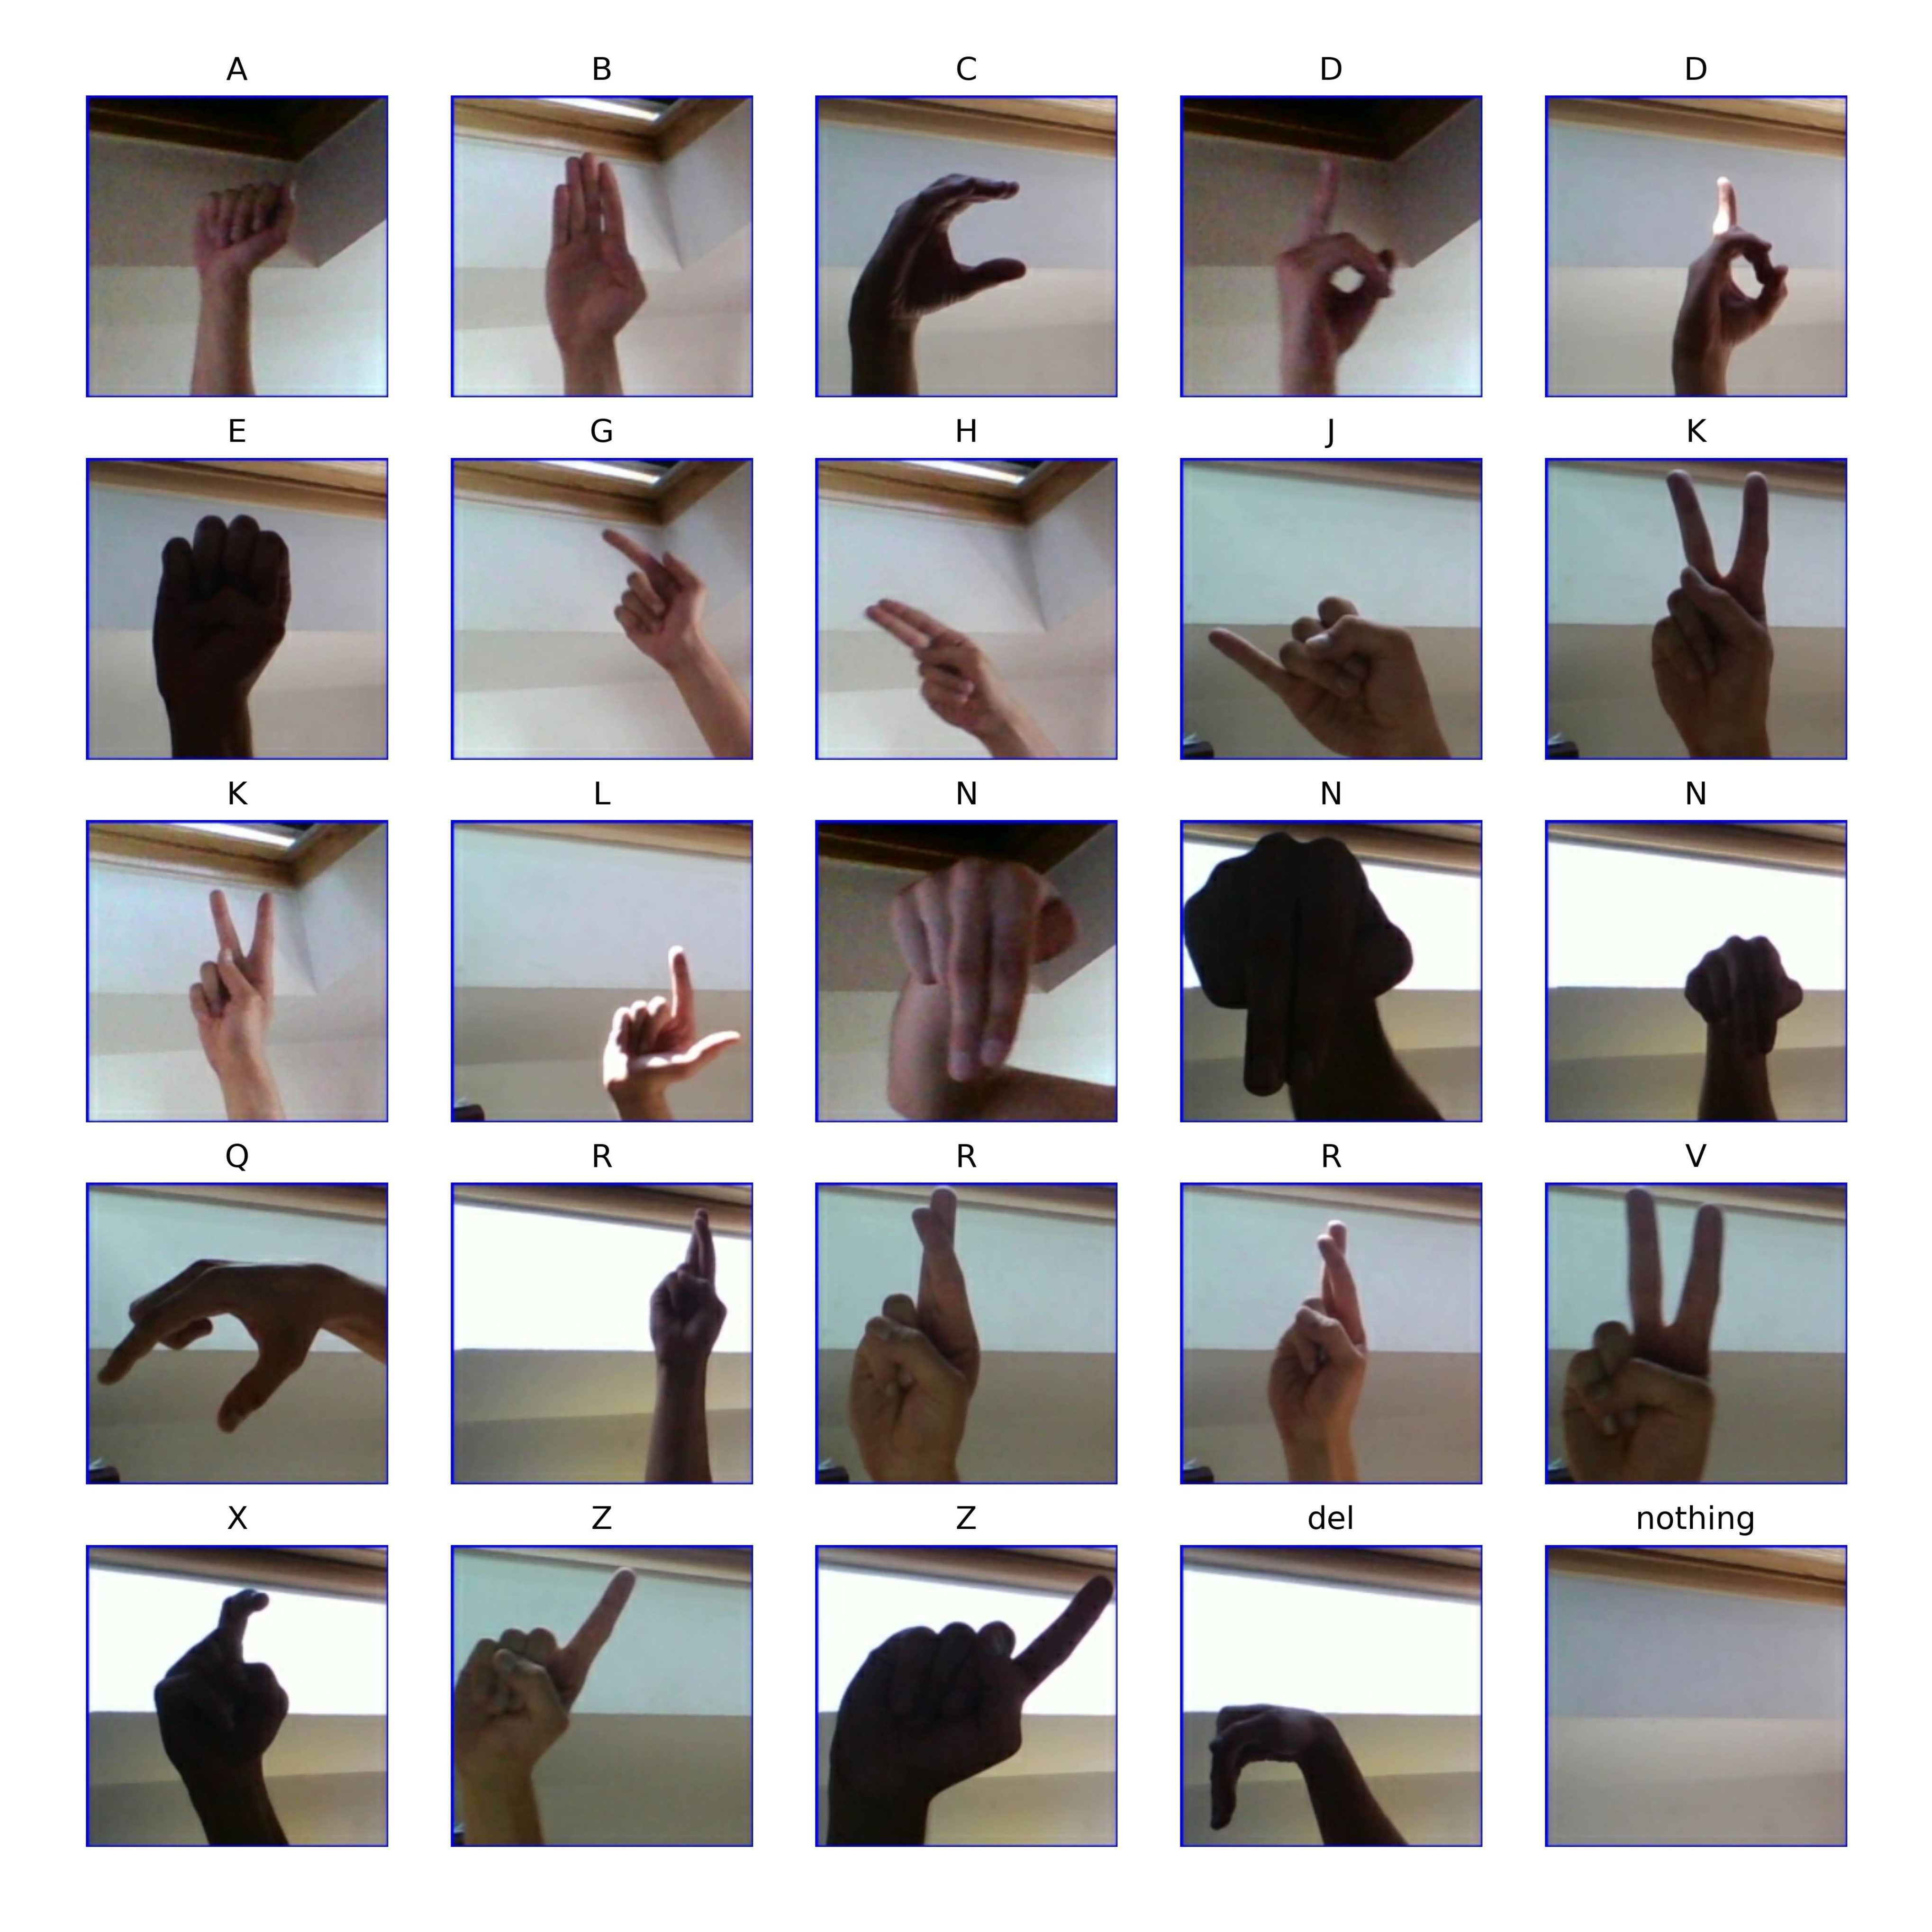
\includegraphics[width=\textwidth]{Figures/eda/asl_samples.jpg}
    \caption{Visualization of 25 samples from the ASL dataset}
    \label{fig:asl_raw}
\end{figure}

Interestingly, we notice that every image presents a blue line around the borders. Worried that this may potentially introduce some bias into the model, we decided to remove this border using TensorFlow. In the following picture, we can see some samples from the pre-processed data.

\begin{figure}[H]
    \centering
    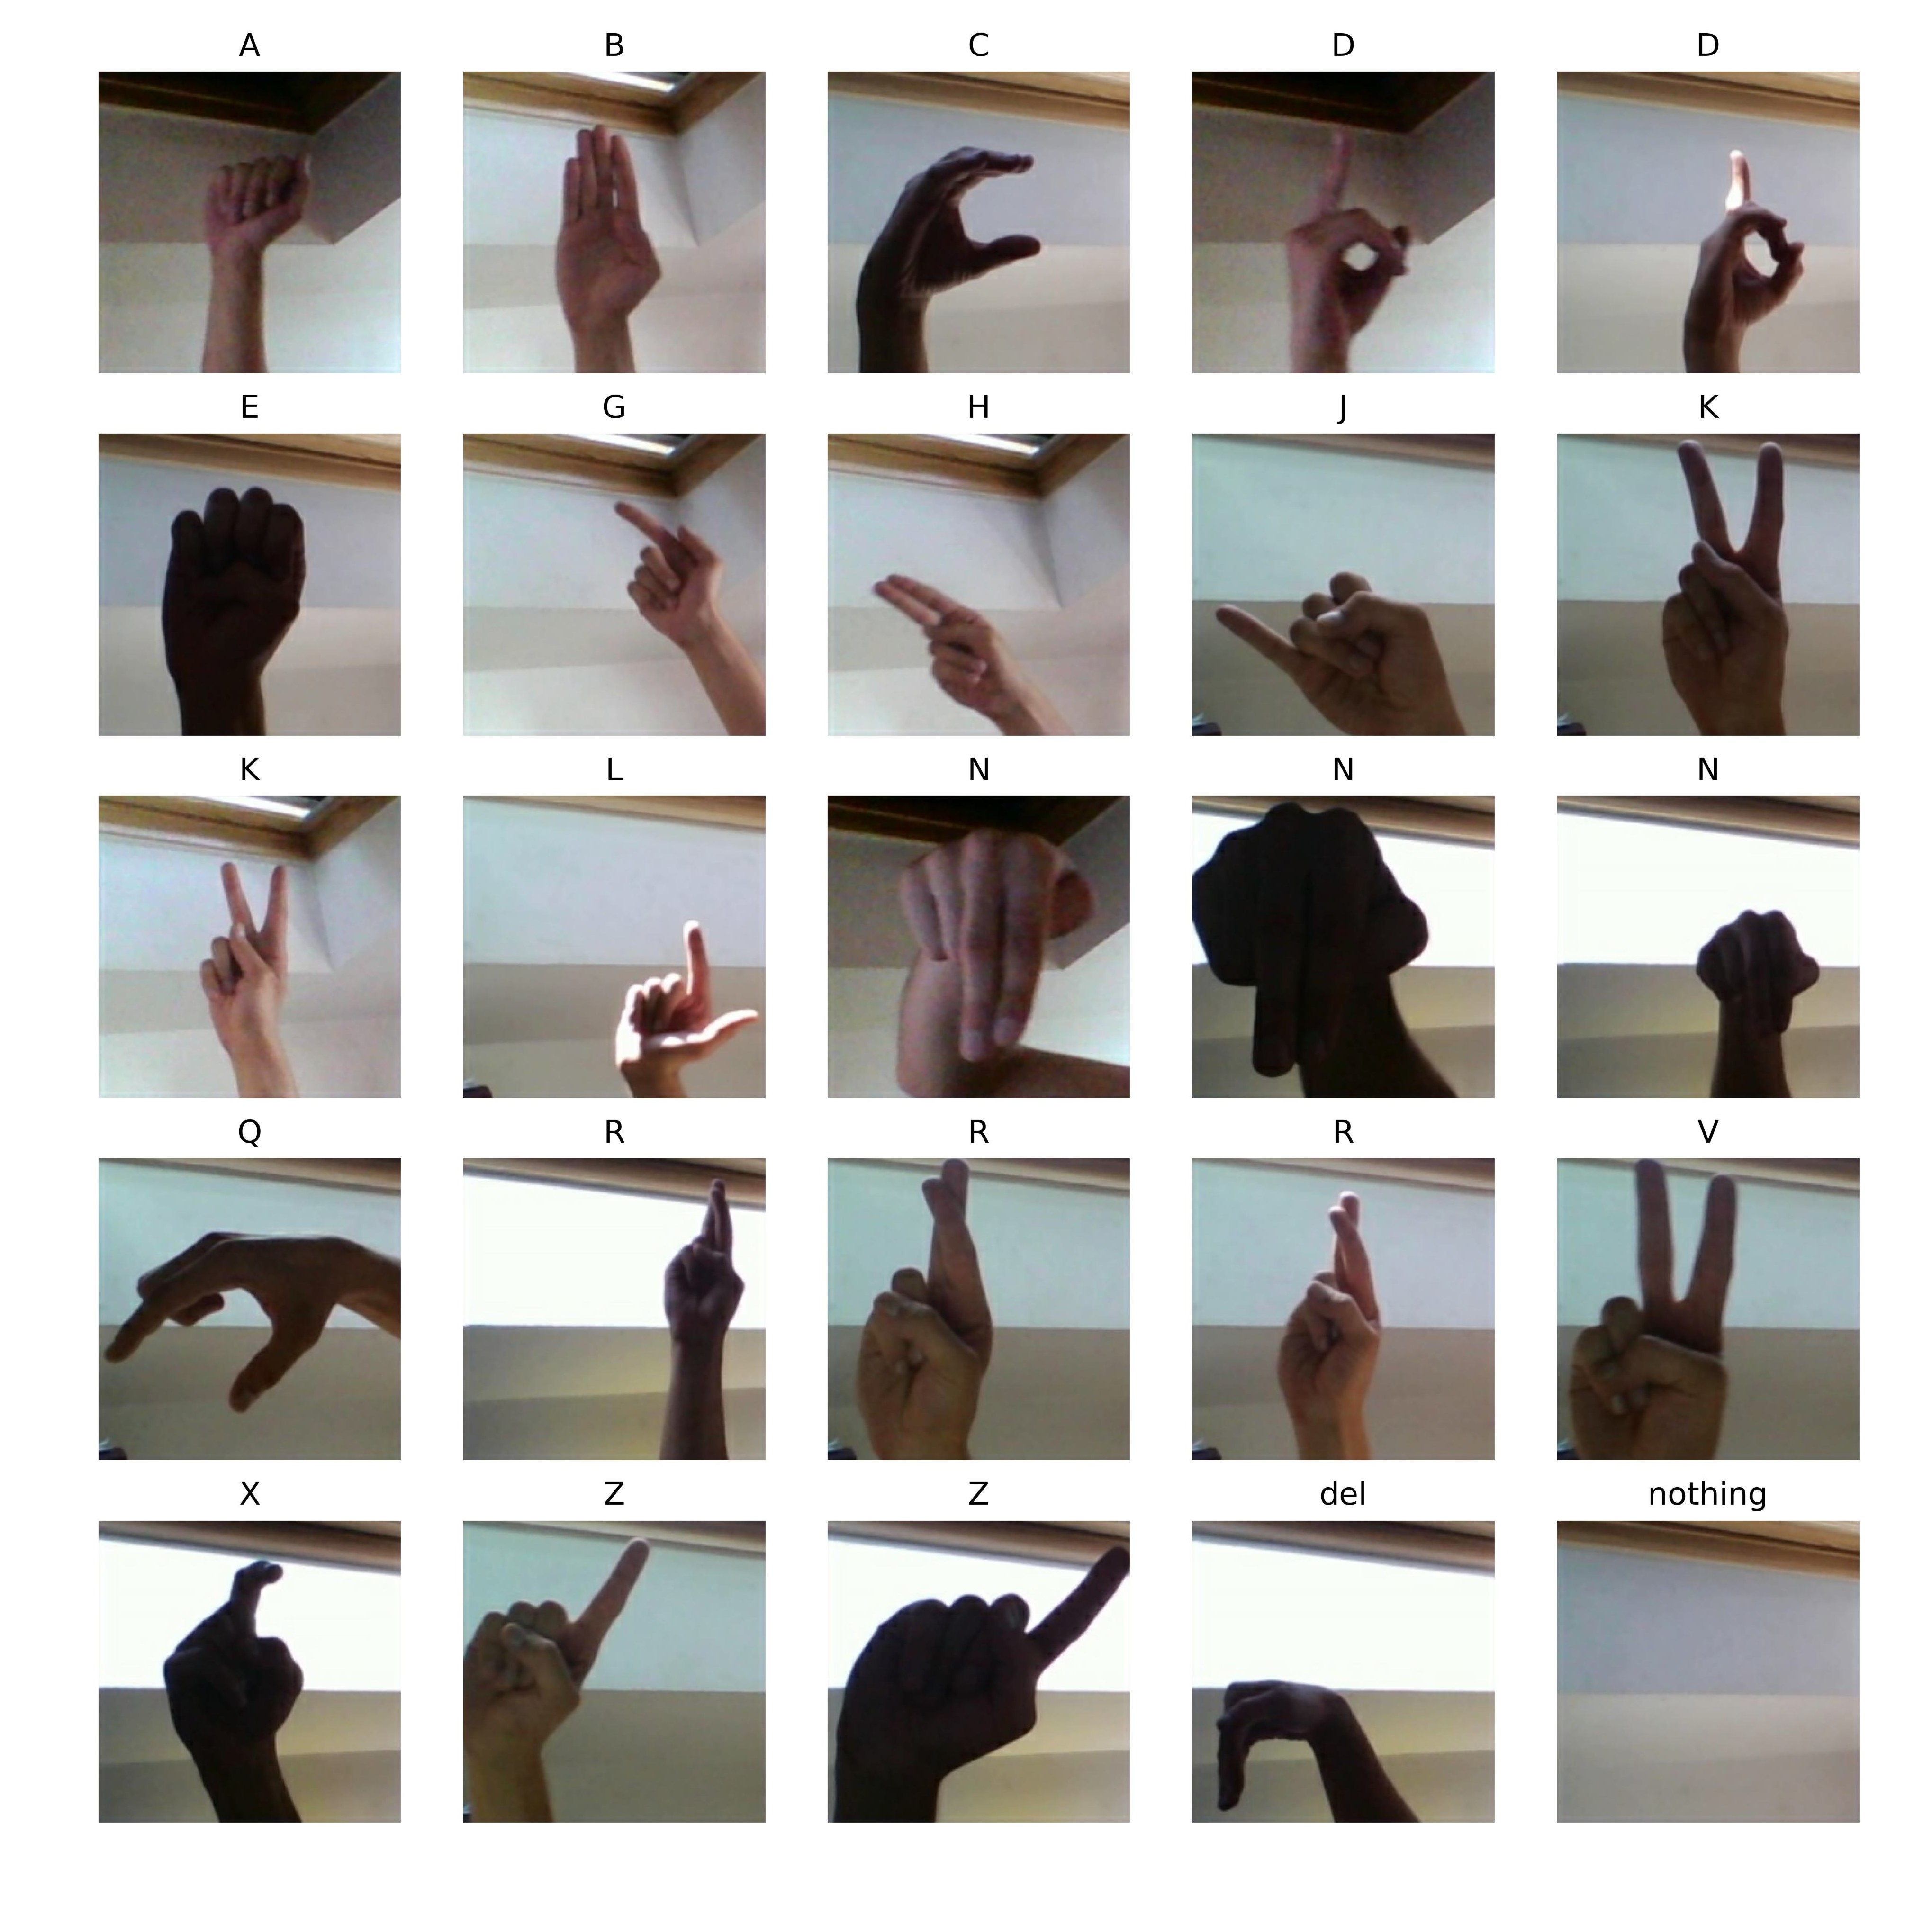
\includegraphics[width=\textwidth]{Figures/eda/asl_samples_processed.jpg}
    \caption{Visualization of 25 samples from the ASL dataset with the blue border removed}
    \label{fig:asl_processed}
\end{figure}

Subsequently,  we have to check that the distribution of the classes is balanced, given that having balanced classes is a good practice when working with a classification problem. 
Fortunately, this dataset presents completely balanced classes, as we can see from the following chart. Hence, no further intervention is necessary.

\begin{figure}[H]
    \centering
    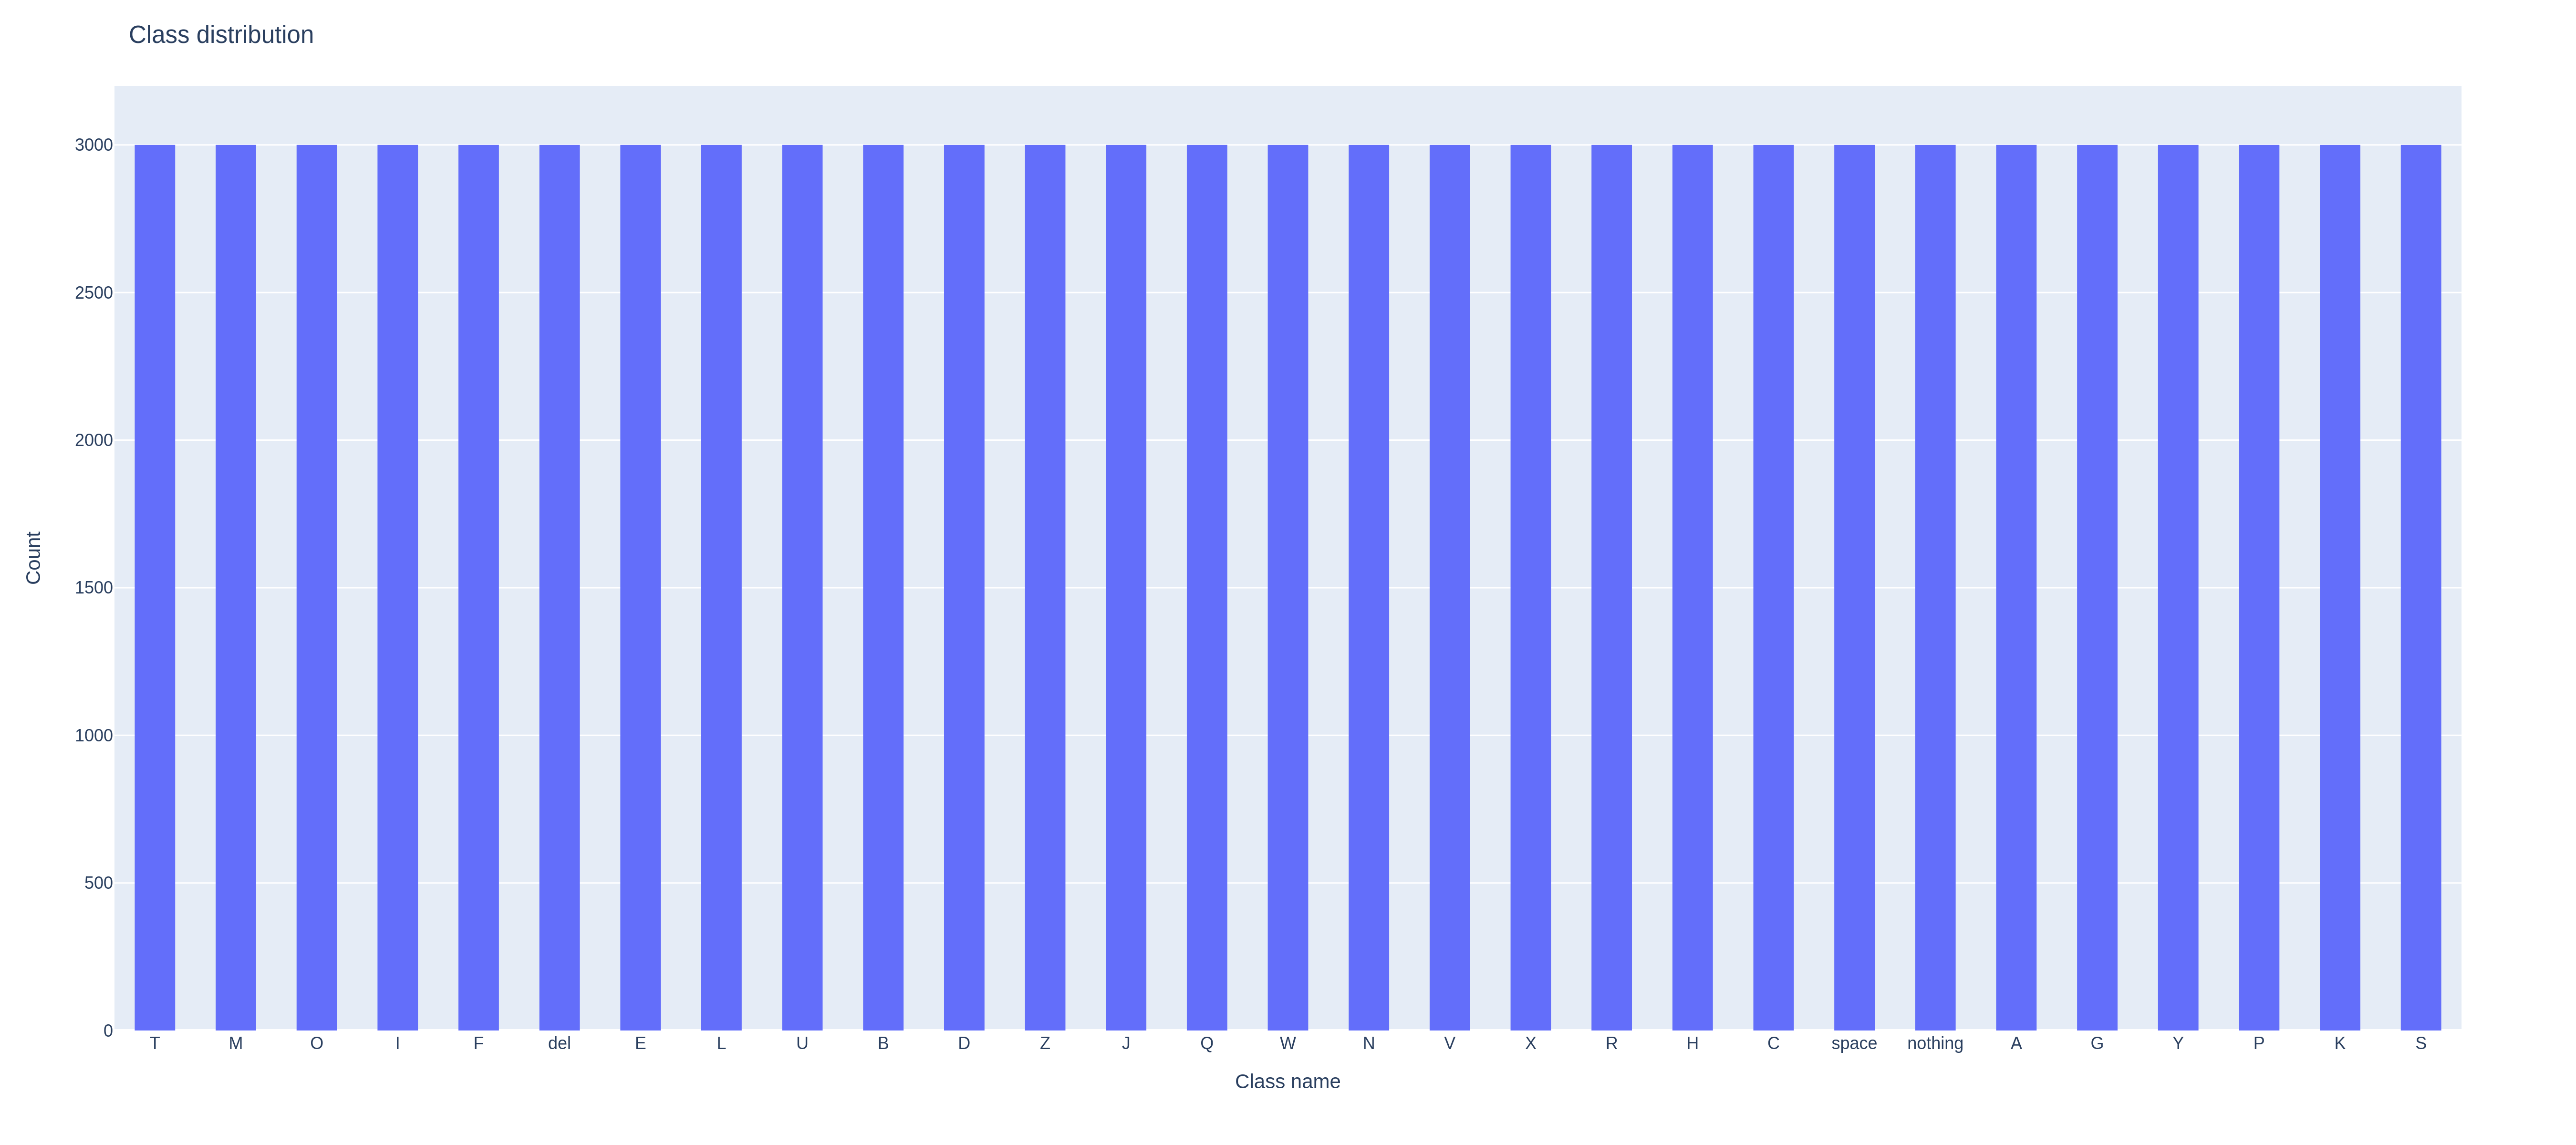
\includegraphics[width=\textwidth]{Figures/eda/class distribution.png}
    \caption{Distribution of the classes of the ASL dataset}
    \label{fig:class_distribution}
\end{figure}


\section{Selecting a subset of the classes}
\label{sec:subset}
The ASL dataset comprises 29 classes. However, there is no need for us to utilize all the classes to develop our hand-gesture recognition system. We do not need to include all 29 distinct gestures, and more importantly, we trust that having fewer classes will benefit the performance of the tiny model we are going to develop. Therefore, our objective is to select a subset of the classes to be kept and used to develop the HGR system.

We want to select a subset of the classes such that the classes inside can be easily distinguished not by a human observer, but from the perspective of a Machine Learning model. 

To determine the optimal subset, we employed three increasingly complex dimensionality reduction techniques:
\begin{itemize}
    \item Principal Component Analysis (PCA)
    \item t-distributed Stochastic Neighbor Embedding (t-SNE)
    \item Feature extraction with a pre-trained CNN
\end{itemize}

Before proceeding, we resized the images to dimensions of 96 x 96 pixels using TensorFlow, given that it is a very common input size for tiny models, and we want to be consistent with the shape of the images that the model will receive as input.

The first two techniques (PCA and t-SNE) require working with grayscale images. We performed the conversion using TensorFlow. We initiated the process with PCA, which is a linear dimensionality reduction technique. In the following image, we can see a scatter plot of the two first principal components of each sample after PCA has been applied. 

\begin{figure}[H]
    \centering
    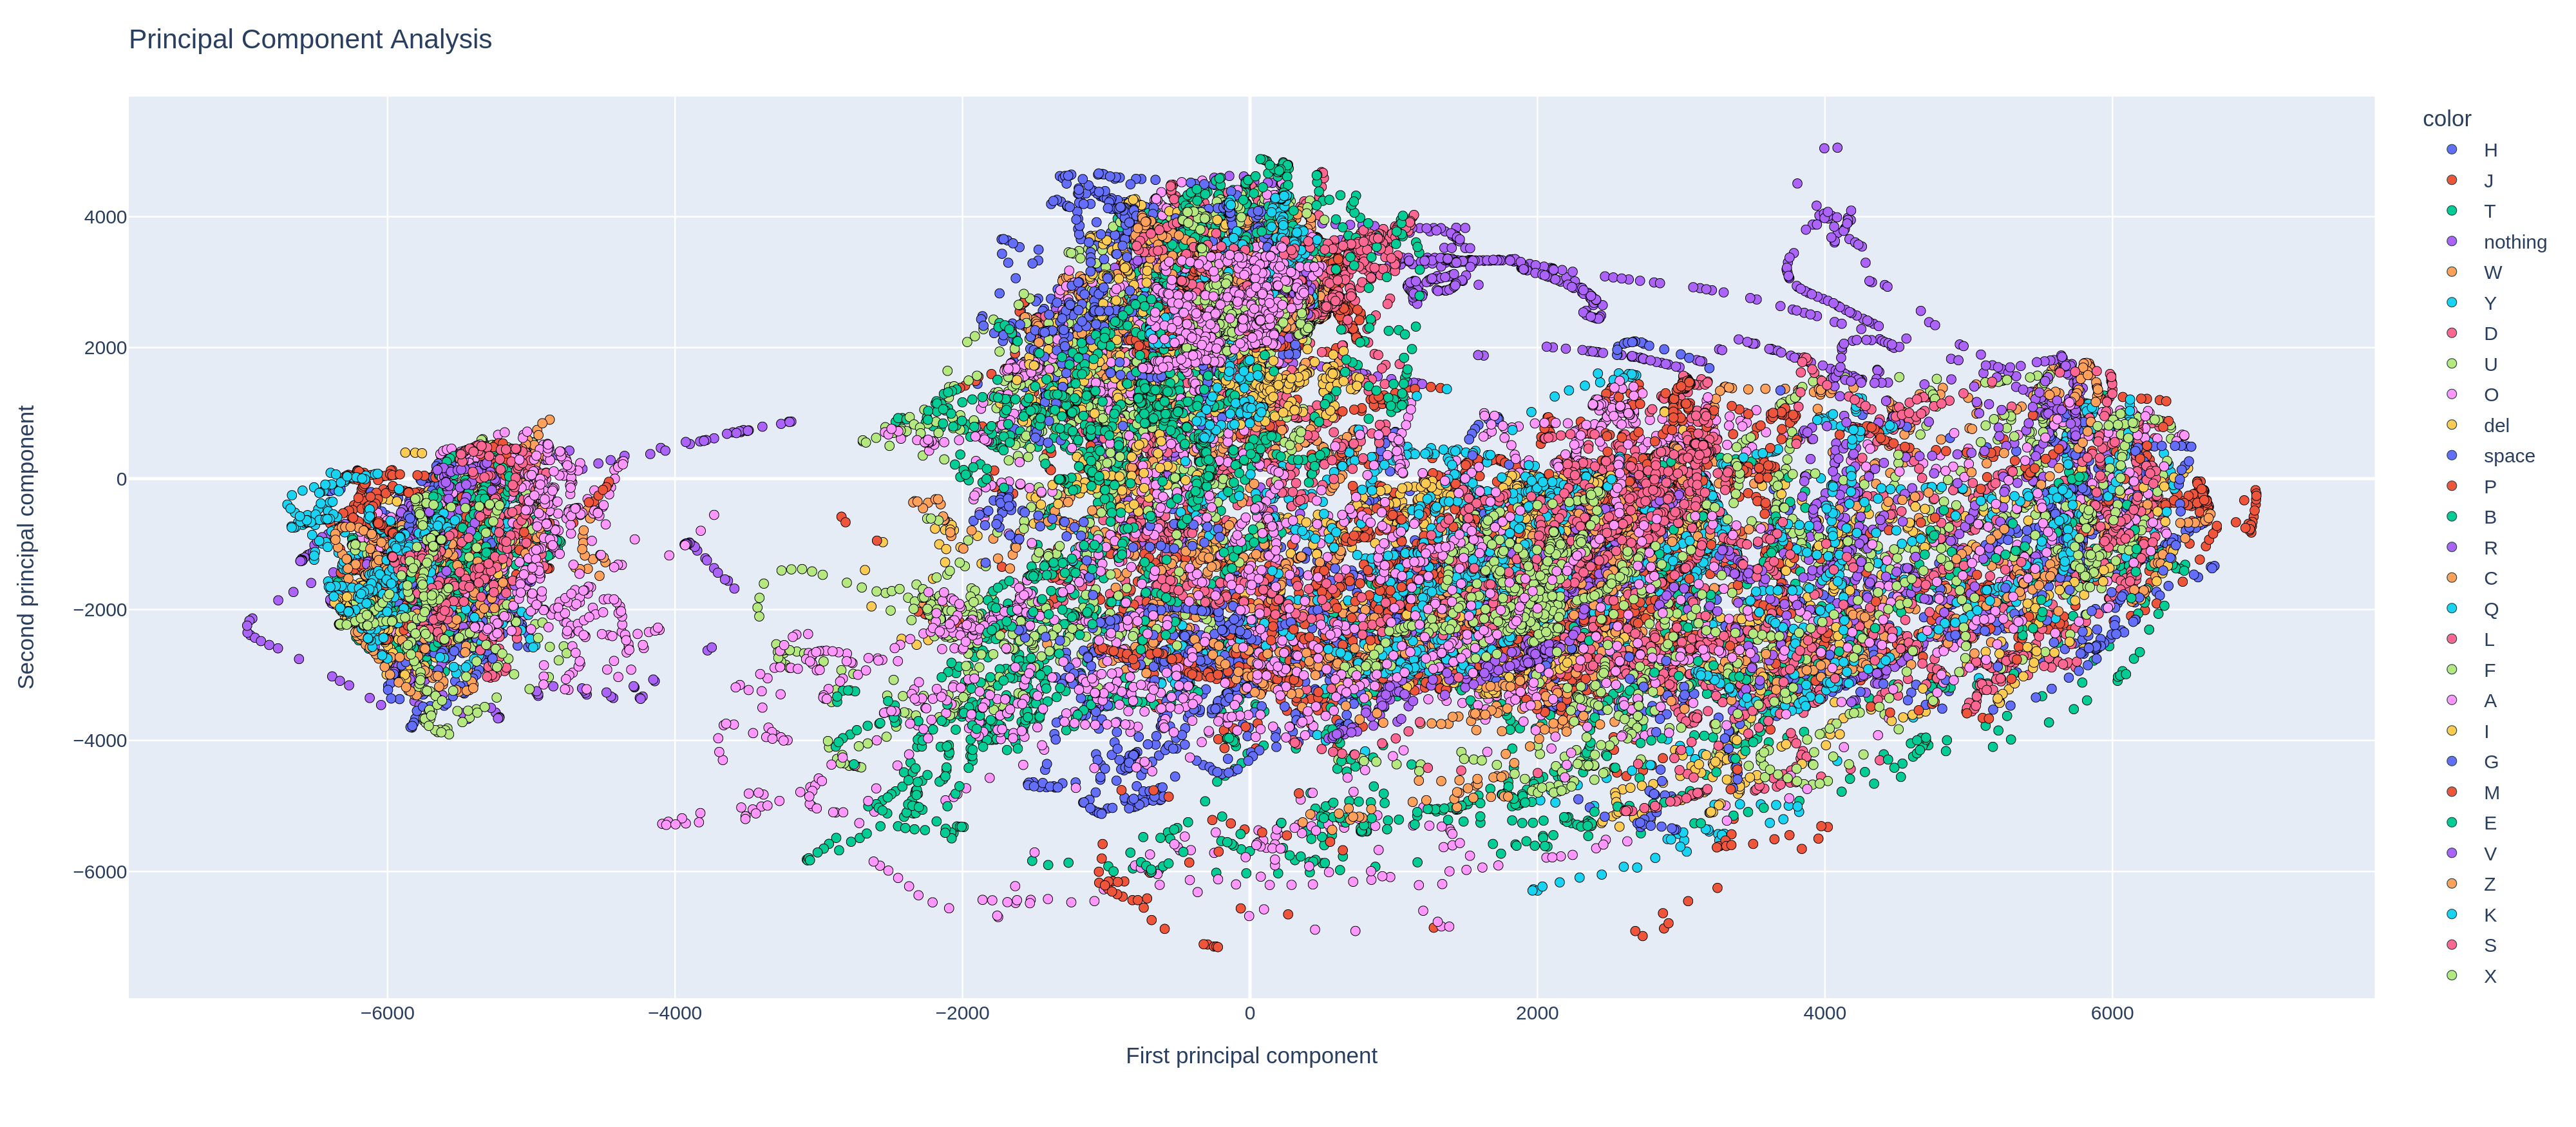
\includegraphics[width=\textwidth]{Figures/eda/pca.png}
    \caption{Scatter plot of the results of the PCA algorithm on the ASL dataset}
    \label{fig:pca}
\end{figure}

The results are far from being useful for our objective. In fact, we did not expect PCA to perform well on highly-dimensional data and unstructured data like images. Therefore, we moved to a different technique, t-SNE, which is known to perform better than PCA because it is non-linear and therefore works better for unstructured real-world data. In the following image, we can see a scatterplot of the first two dimensions after t-SNE has been applied. 

\begin{figure}[H]
    \centering
    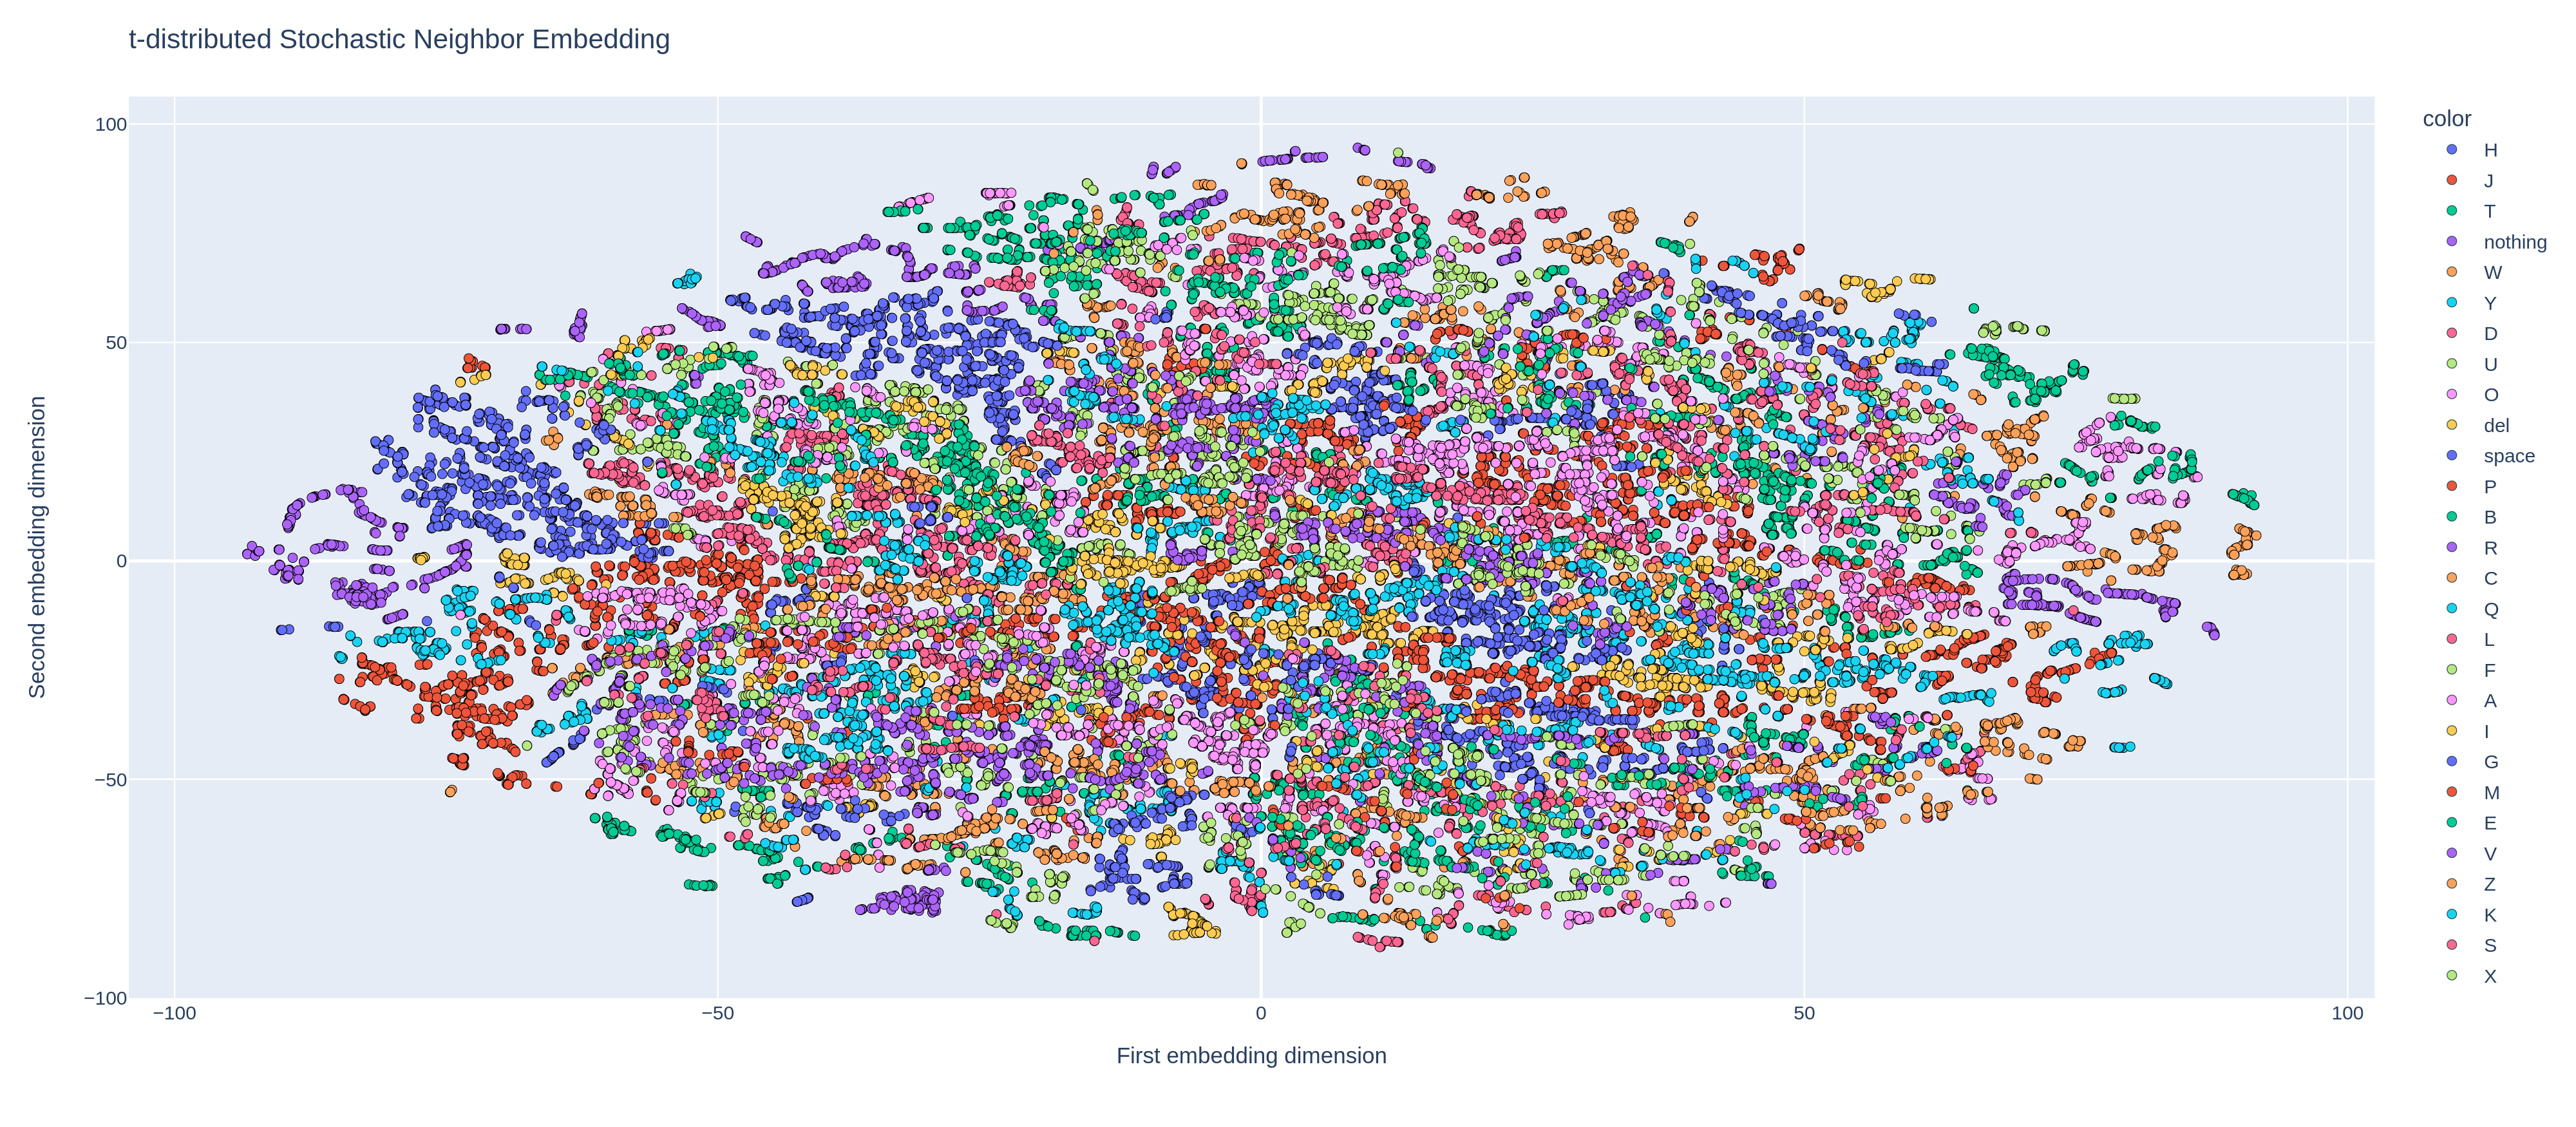
\includegraphics[width=\textwidth]{Figures/eda/tsne.png}
    \caption{Scatter plot of the results of the t-SNE algorithm on the ASL dataset}
    \label{fig:tsne}
\end{figure}

It is worth noting that the t-SNE algorithm is computationally intensive and generally not recommended for data exceeding 50 dimensions. However, we were able to apply it regardless of our setting thanks to the RAPIDS cuML library \cite{cuml} that allows us to perform the computation of the algorithm directly on the GPU, accelerating to a few seconds what would otherwise have taken multiple hours on the CPU.

Still, the results are of no interest to us since the scatter plot does not enable us to discern the class structure. Thus, in our final attempt, we decided to perform feature extraction using a pre-trained CNN.  This approach offers the advantage of operating directly on RGB images (thereby processing more information) and yielding a more compact data representation. Subsequently, t-SNE can be applied to this representation for further dimensionality reduction and to make creating a visualization possible.

The model we are using as a feature extractor is EfficientNetV2B1, pre-trained on ImageNet. It is one of the models with the highest top-5 accuracy available on Keras and that does not take too long to process the images. We removed the classification head of the model and kept only the global feature extraction part. For each image, the model will output a feature vector with 1280 dimensions. In the following image, we can see a scatterplot of the first two dimensions after t-SNE has been applied.

\begin{figure}[H]
    \centering
    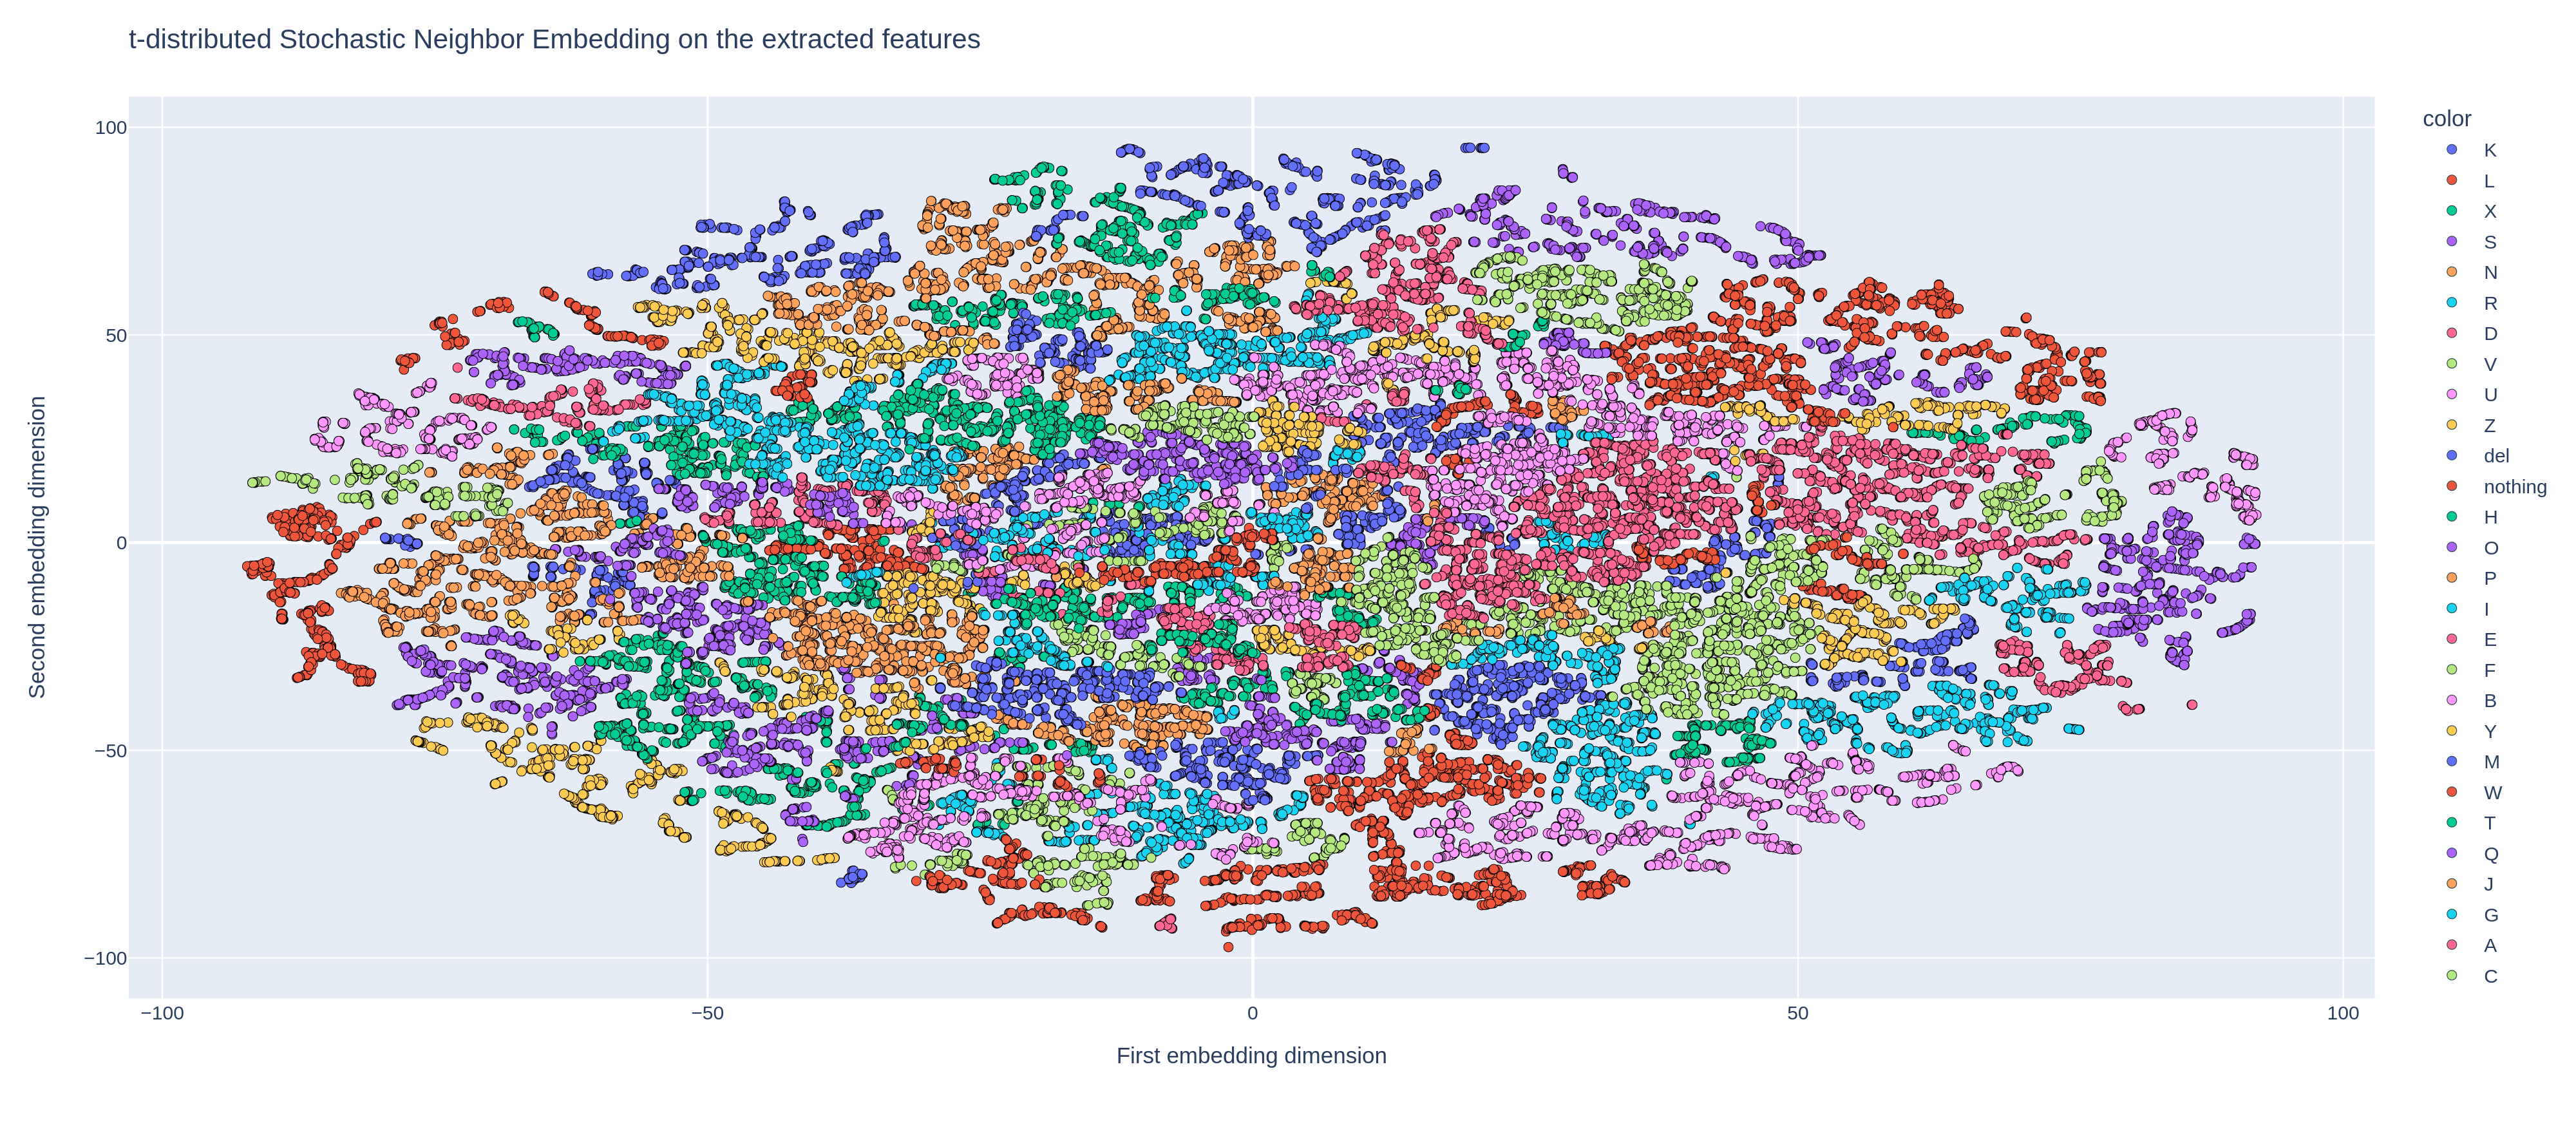
\includegraphics[width=\textwidth]{Figures/eda/cnn_tsne.png}
    \caption{Scatter plot of the results of the t-SNE algorithm on the features extracted from the ASL dataset}
    \label{fig:cnn_tsne}
\end{figure}

This time, the data exhibits a more discernible structure. Nonetheless, identifying the most distinguishable and classifiable group of classes remains challenging. Therefore, instead of relying on dimensionality reduction techniques, we decided to first train a model to classify all 29 classes, check its performance on each class, and then keep only the classes with the highest performance. A more detailed description of this process is covered in the following chapter.


\chapter{All-gestures Model}
\label{ch:all-model}%
In this chapter, we discuss how the neural network to be deployed on the Arduino device was trained. We refer to this model as \textit{all-gestures} model since it is meant to address a multi-class classification problem on all 29 classes of gestures. 

Every part of this analysis was performed using TensorFlow. The source code can be found in the notebook \textit{all-gestures model.ipynb }of the GitHub repository. 

\section{Model architecture}
\label{sec:all-arch}
Following the Transfer Learning paradigm, which consists of taking features learned on one problem, and leveraging them on a new problem through a pre-trained model, the selection of the architecture falls back into choosing an appropriate pre-trained model, referred to as the \textit{base} model.

The severe memory constraints of the target device greatly reduce the number of Convolutional Neural Network (CNN) architectures that we can choose the \textit{base} model from. In particular, considering the device's mere 256 KB RAM, which also has to be shared with input storage, intermediate feature maps, libraries, and firmware, it is reasonable to say that the final model must not be heavier than approximately 150 KB. 

In order to choose the architecture, we took inspiration from the pre-trained models available on Edge Impulse. Some of them are displayed in the following image.

\begin{figure}[H]
    \centering
    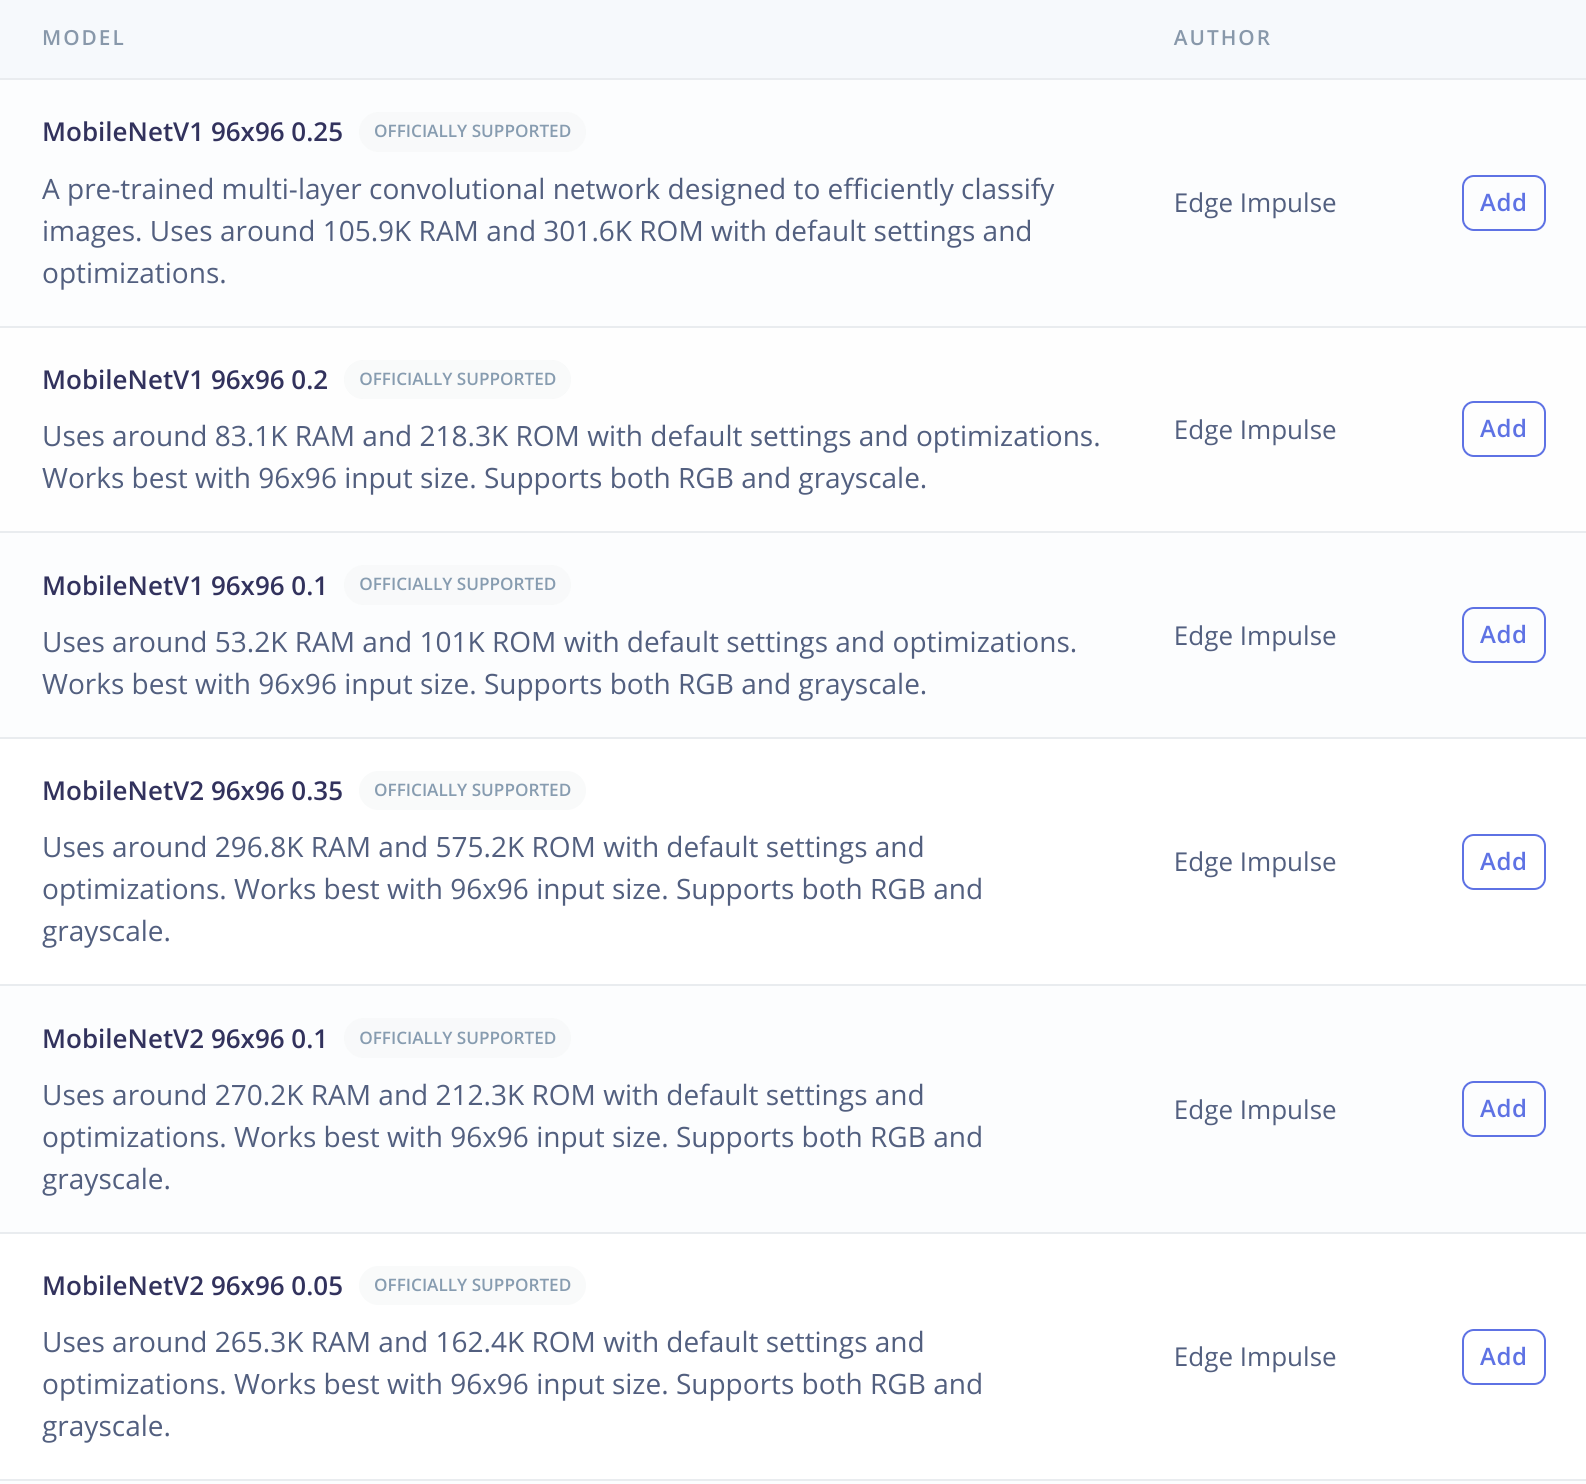
\includegraphics[width=0.9\textwidth]{Figures/edge_impulse_models.png}
    \caption{Some of the available pre-trained models from Edge Impulse.}
    \label{fig:ei_models}
\end{figure}

According to Edge Impulse's estimates, the only architecture that could fit on the 256 KB of RAM of our device is MobileNetV1. Consequently, we decided to proceed with the variant of this architecture with the largest width multiplier $\alpha$ that could fit in our device, which is $\alpha = 0.25$.

Replicating Edge Impulse's MobileNetV1 96x96 0.25 architecture locally was preferred. Local training offers the advantages of faster training times (using GPUs) and extended training duration compared to Edge Impulse's 20-minute free plan limit, which was required in our setting since we are working with a dataset of a very large size.

\begin{figure}[H]
    \centering
    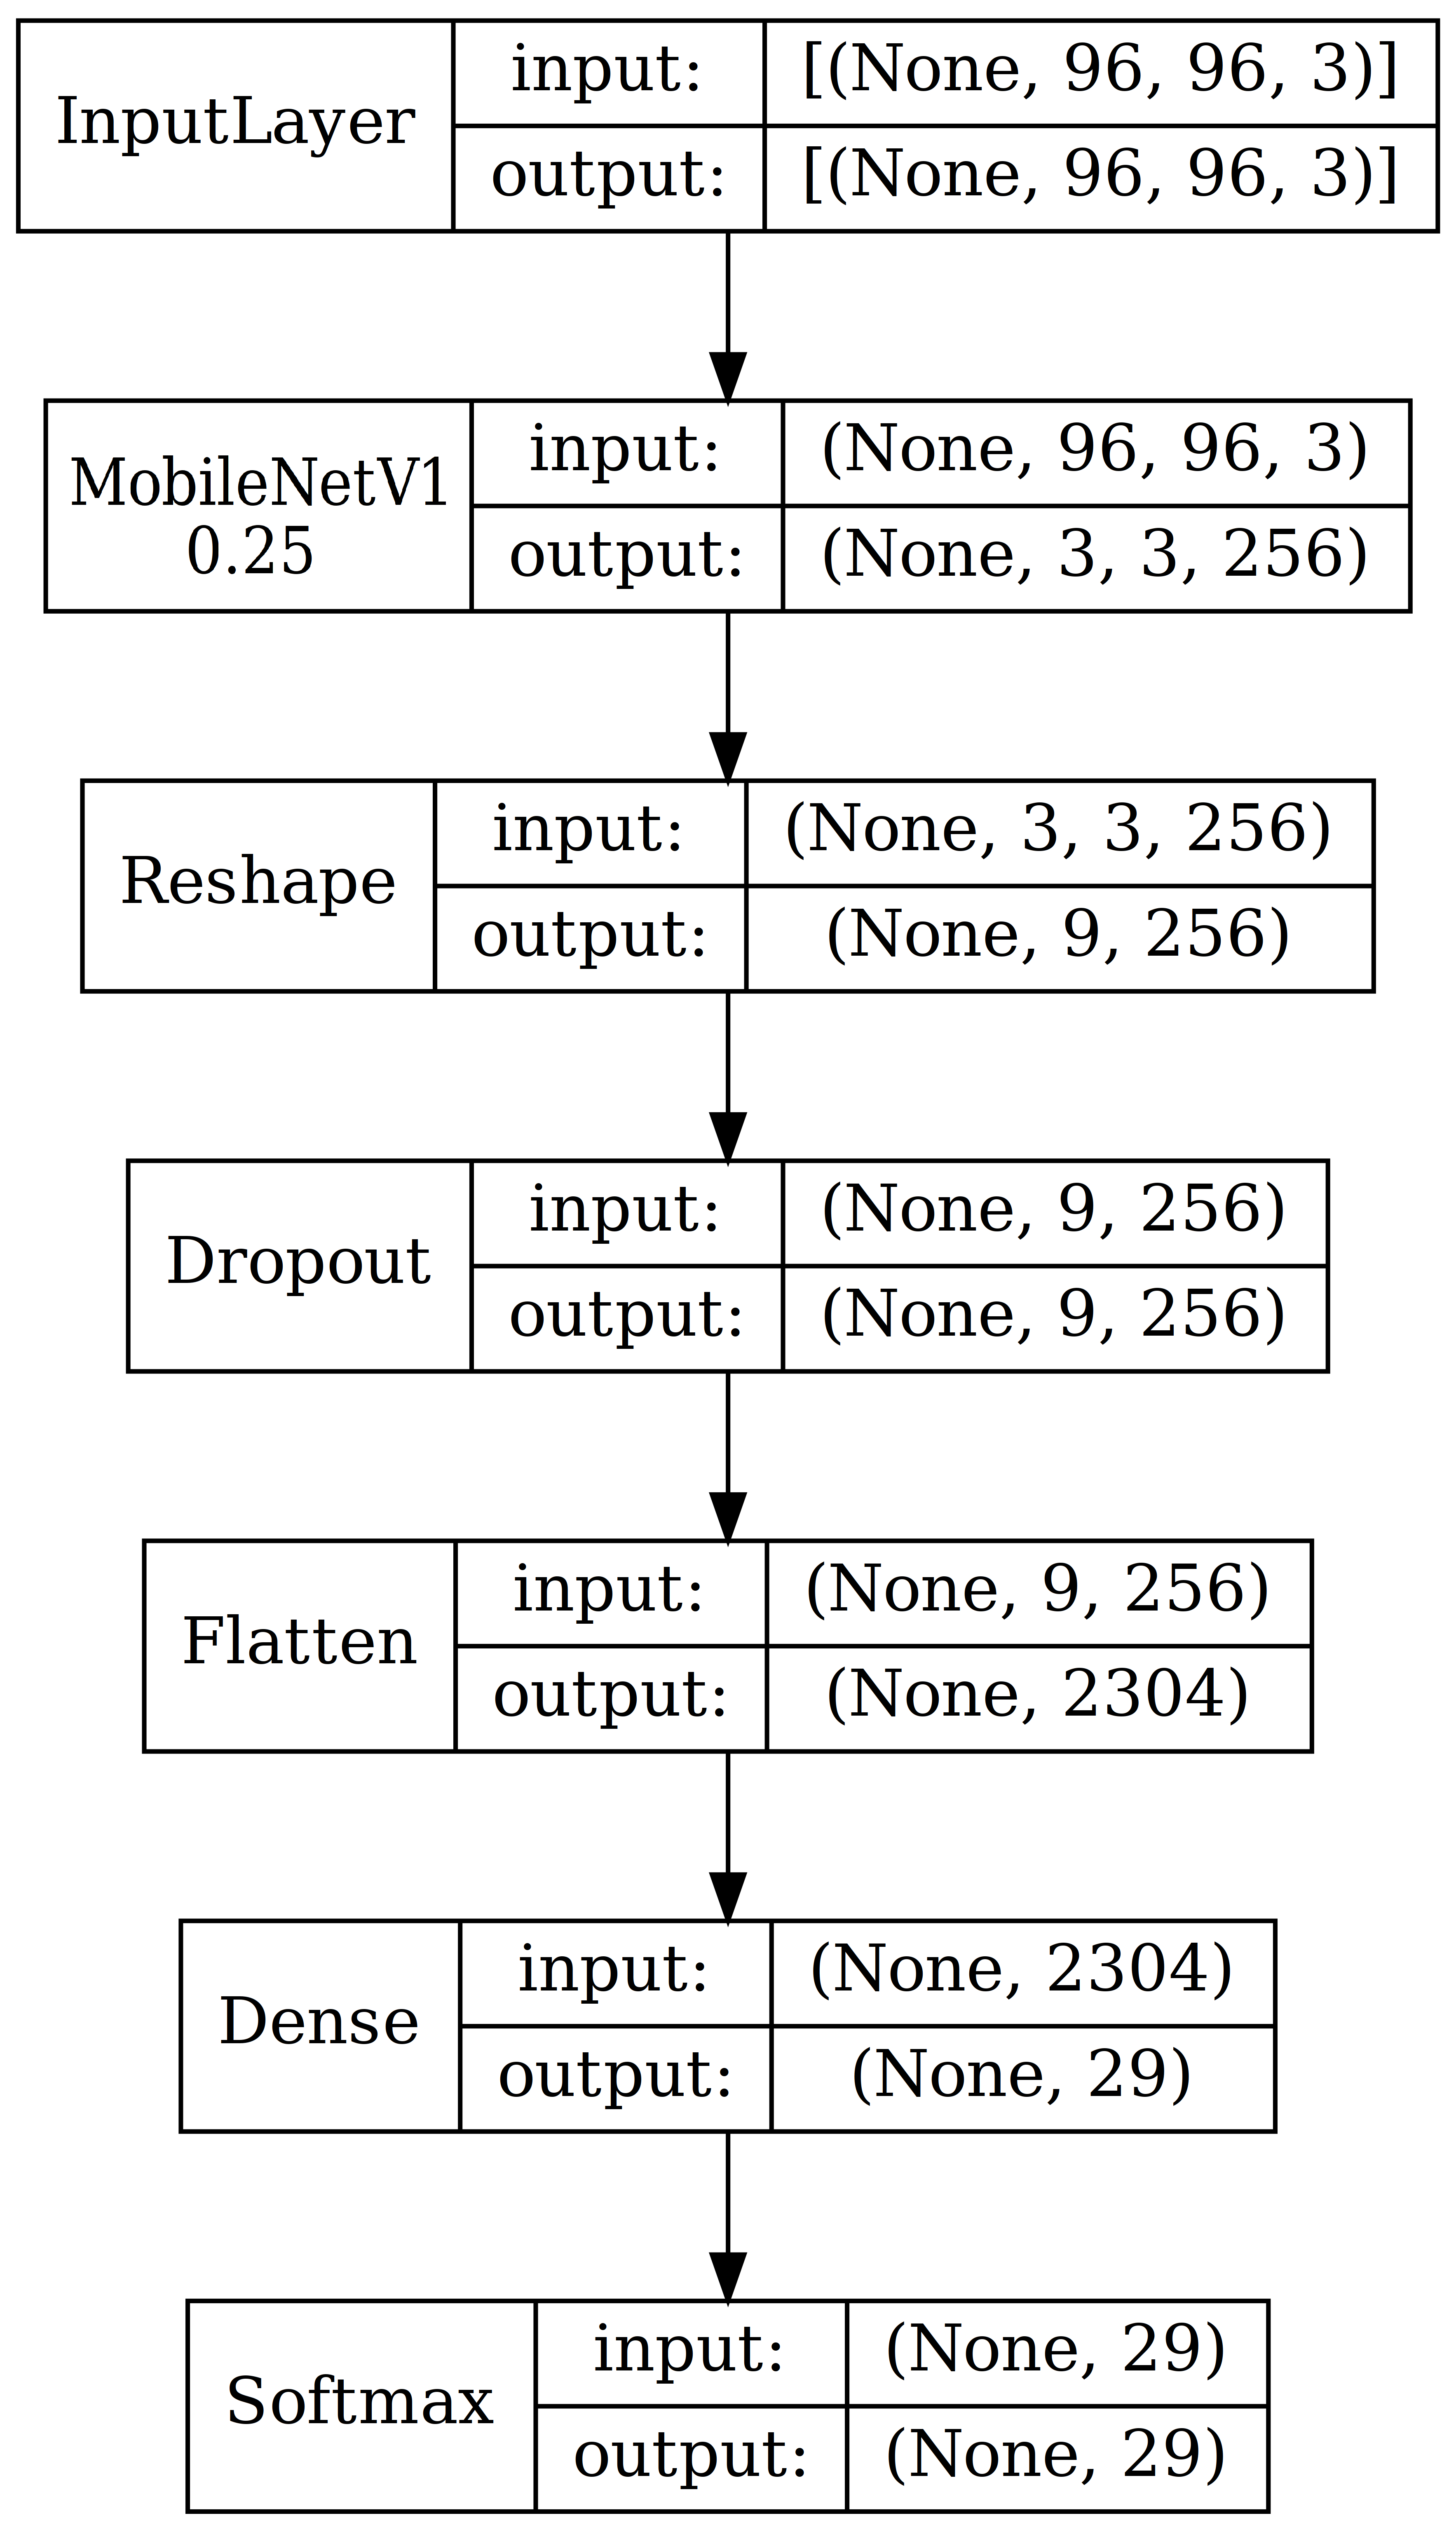
\includegraphics[width=0.35\textwidth]{Figures/all-gestures/all_model.png}
    \caption{The architecture of the \textit{all-gestures} model, with a focus on the layer type and on the input and output shapes.}
    \label{fig:all_architecture}
\end{figure}

\section{Model training}
\label{sec:all-training}
With Transfer Learning, model training comprises two phases: the \textit{fit} phase, where the base model is frozen, and only the dense classifier is trained; and the \textit{fine-tuning} phase, where both the base model and classifier are trained.

In both steps, we are using the Adam optimizer and the Sparse Categorical Cross Entropy loss function in order to perform the gradient descent and the back-propagation. 

For the \textit{fit} phase, we are using an initial learning rate of $0.001$ and training for $20$ epochs. For the \textit{fine-tuning} phase, we are using a much smaller learning rate of $0.00001$ in order to avoid the phenomenon called catastrophic forgetting on the weights of the base model, and training for $20$ epochs.

The final results of the training, i.e. the results of the \textit{fine-tuning} phase, are displayed in the following charts.
\begin{figure}[H]
    \centering
    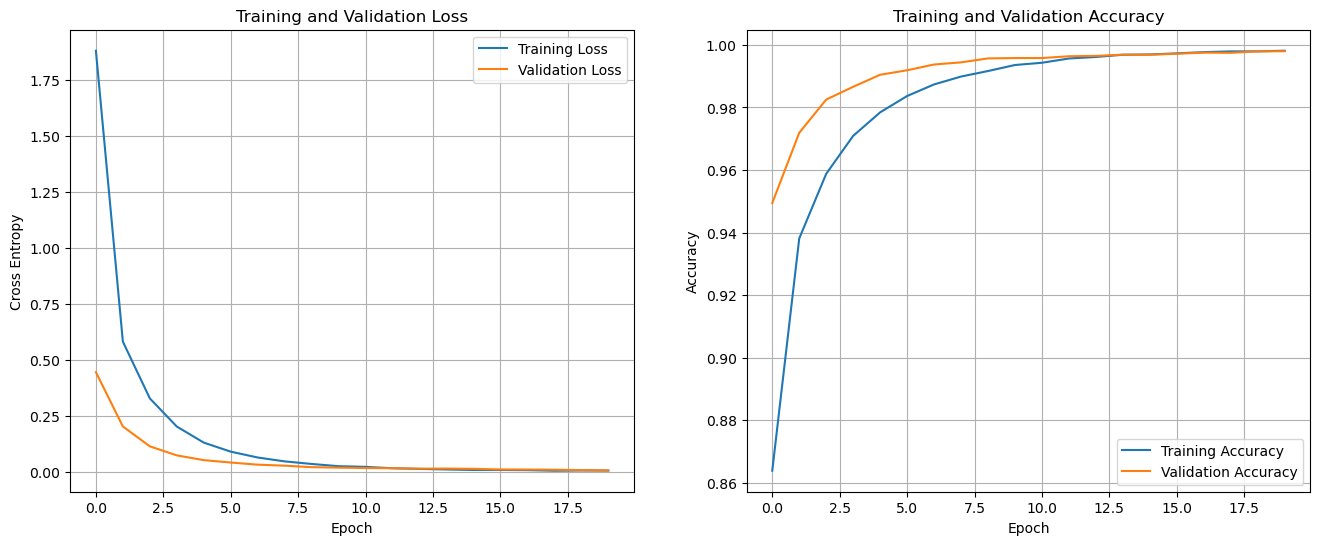
\includegraphics[width=\textwidth]{Figures/all-gestures/all_loss.png}
    \caption{Evolution of the loss function and of the accuracy of the \textit{all-gestures} model on both the training and the validation sets.}
    \label{fig:all_loss}
\end{figure}


\section{Model evaluation}
\label{sec:all-evaluation}
In this section we take a closer look at the performance of the trained model, focusing on the validation set only. From the previous figure, we can see that the model achieved an extremely high performance since it was able to reach an accuracy very close to 100\% without overfitting. 

Satisfied with this result, our next step is to take a look at which are the classes in which the model performs better, as anticipated in the section \ref{sec:subset}.  In order to do so, we can evaluate the model on the full validation set and generate a confusion matrix, which will highlight the samples for which the model ends up with an incorrect prediction. Then, from the confusion matrix we can compute the number of errors for each class, and finally normalize it on the number of samples for each class.

Consequently, we can easily visualize the results by using a bar plot. 

\begin{figure}[H]
   \centering
   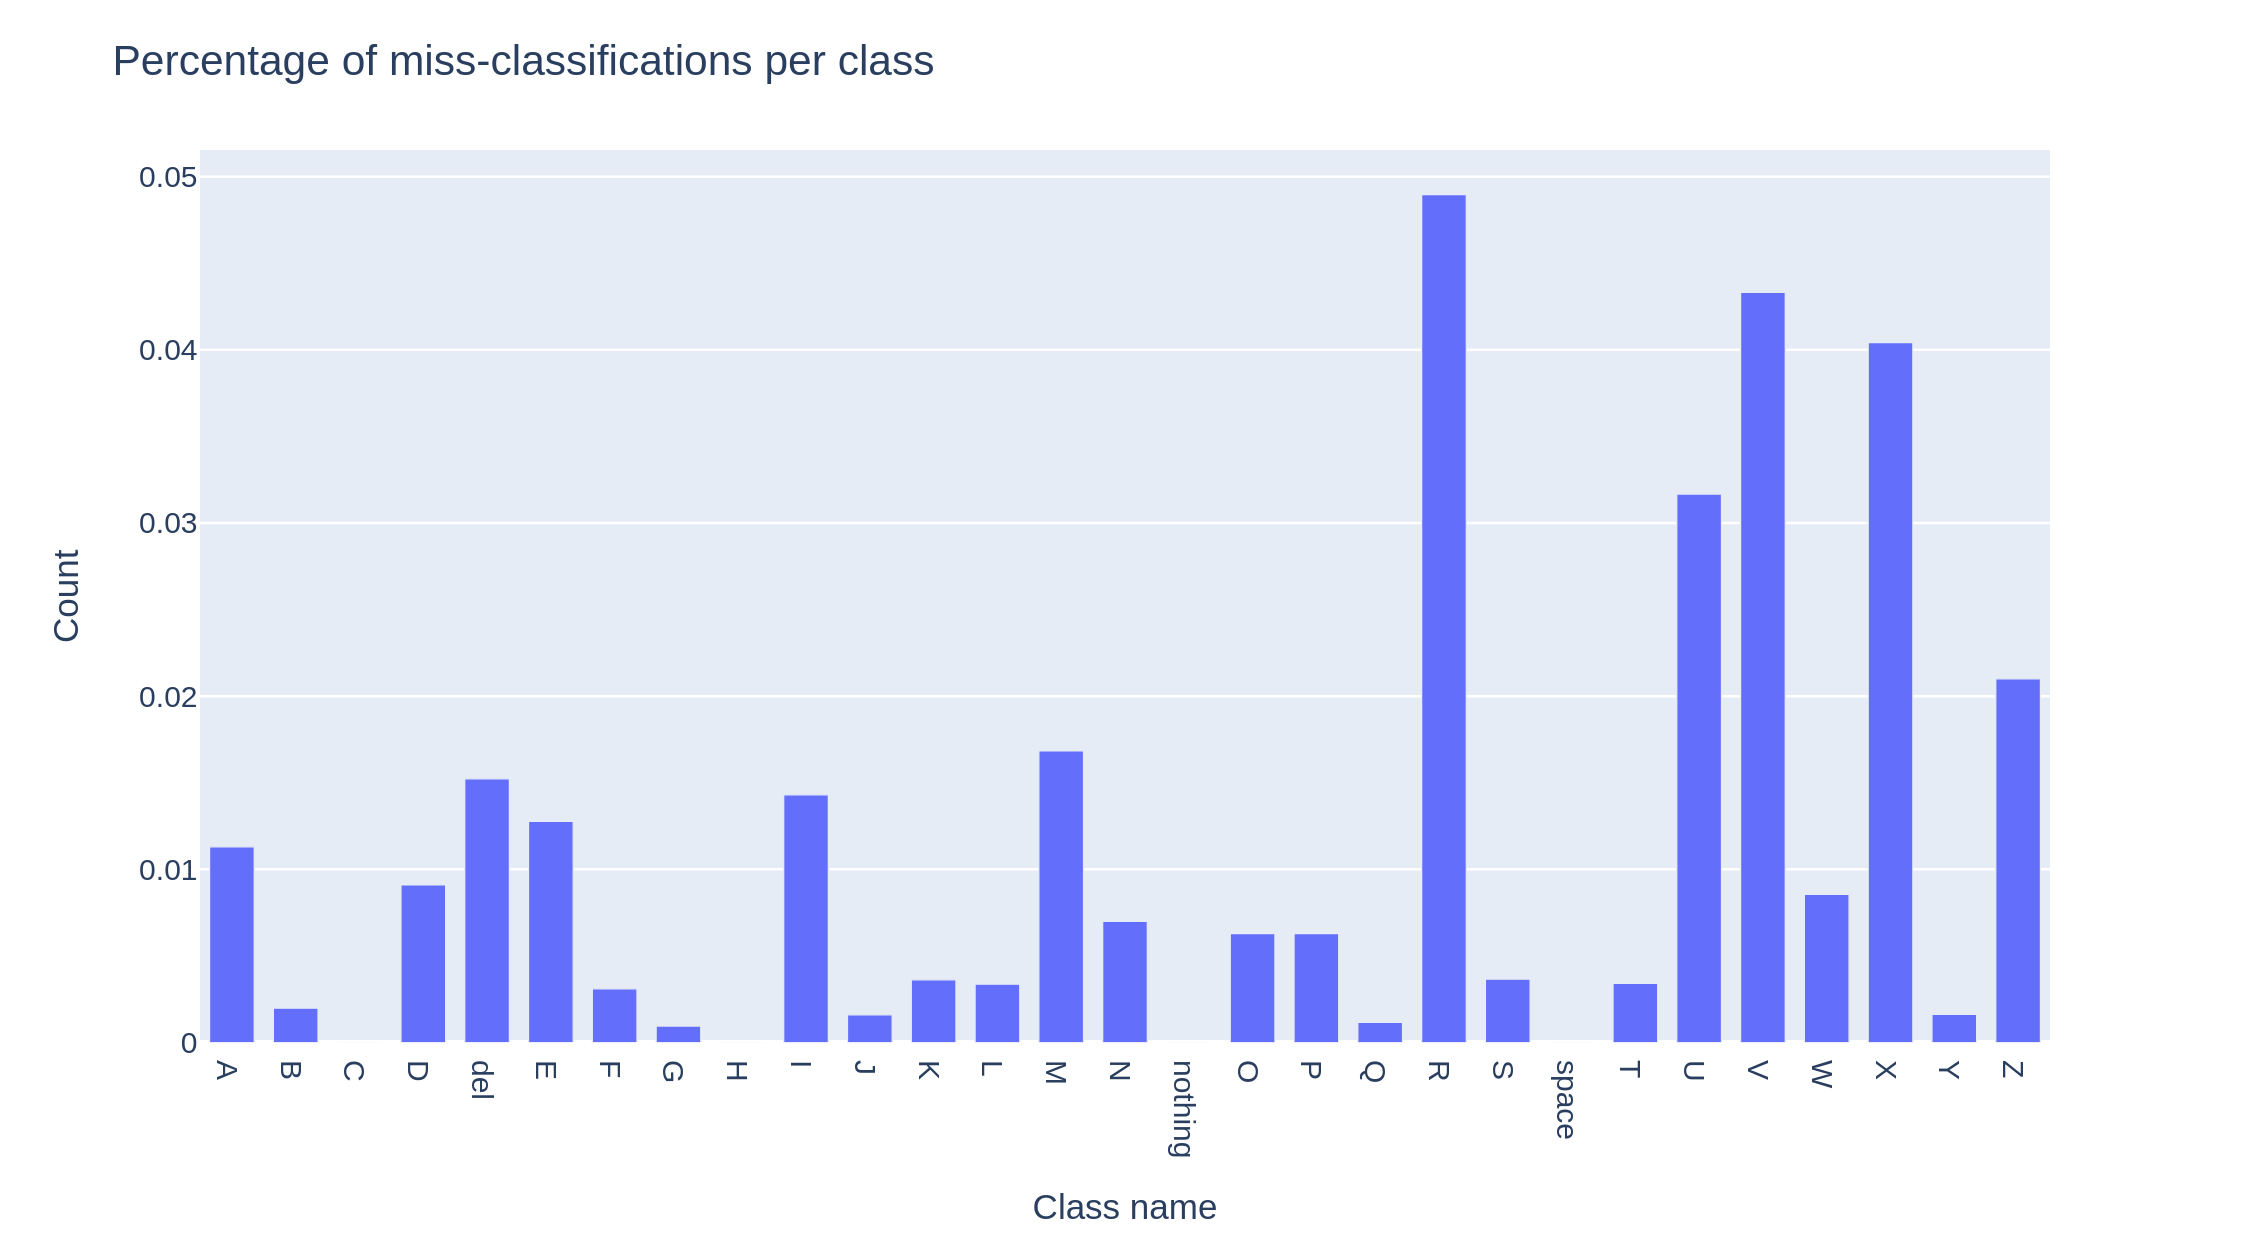
\includegraphics[width=\textwidth]{Figures/all-gestures/all_errors.png}
   \caption{Percentage of miss-classification per class of the \textit{all-gestures} model.}
   \label{fig:all_errors}
\end{figure}

From the chart above, we can see that the model performs very well with the classes \textit{C}, \textit{G}, \textit{H}, \textit{Q} and \textit{space}. We will also include the \textit{nothing} class as it can be very useful in real-world applications to detect the absence of gestures or hands.


\chapter{5-gestures Model}
\label{ch:5-model}%
Now that we have selected a good subset of the classes, we can keep these only and train a very similar model to the one in the previous chapter. This is the model that will be deployed on the device and is referred to as \textit{5-gestures} model. 

Every part of this analysis was performed using TensorFlow. The source code can be found in the notebook \textit{5-gestures model.ipynb} of the GitHub repository. 


\section{Model architecture}
\label{sec:5-arch}
The architecture of the \textit{5-gestures} model mirrors the \textit{all-gestures} model, with adaptations in the dense classifier to accommodate the 6 selected classes.

\begin{figure}[H]
    \centering
    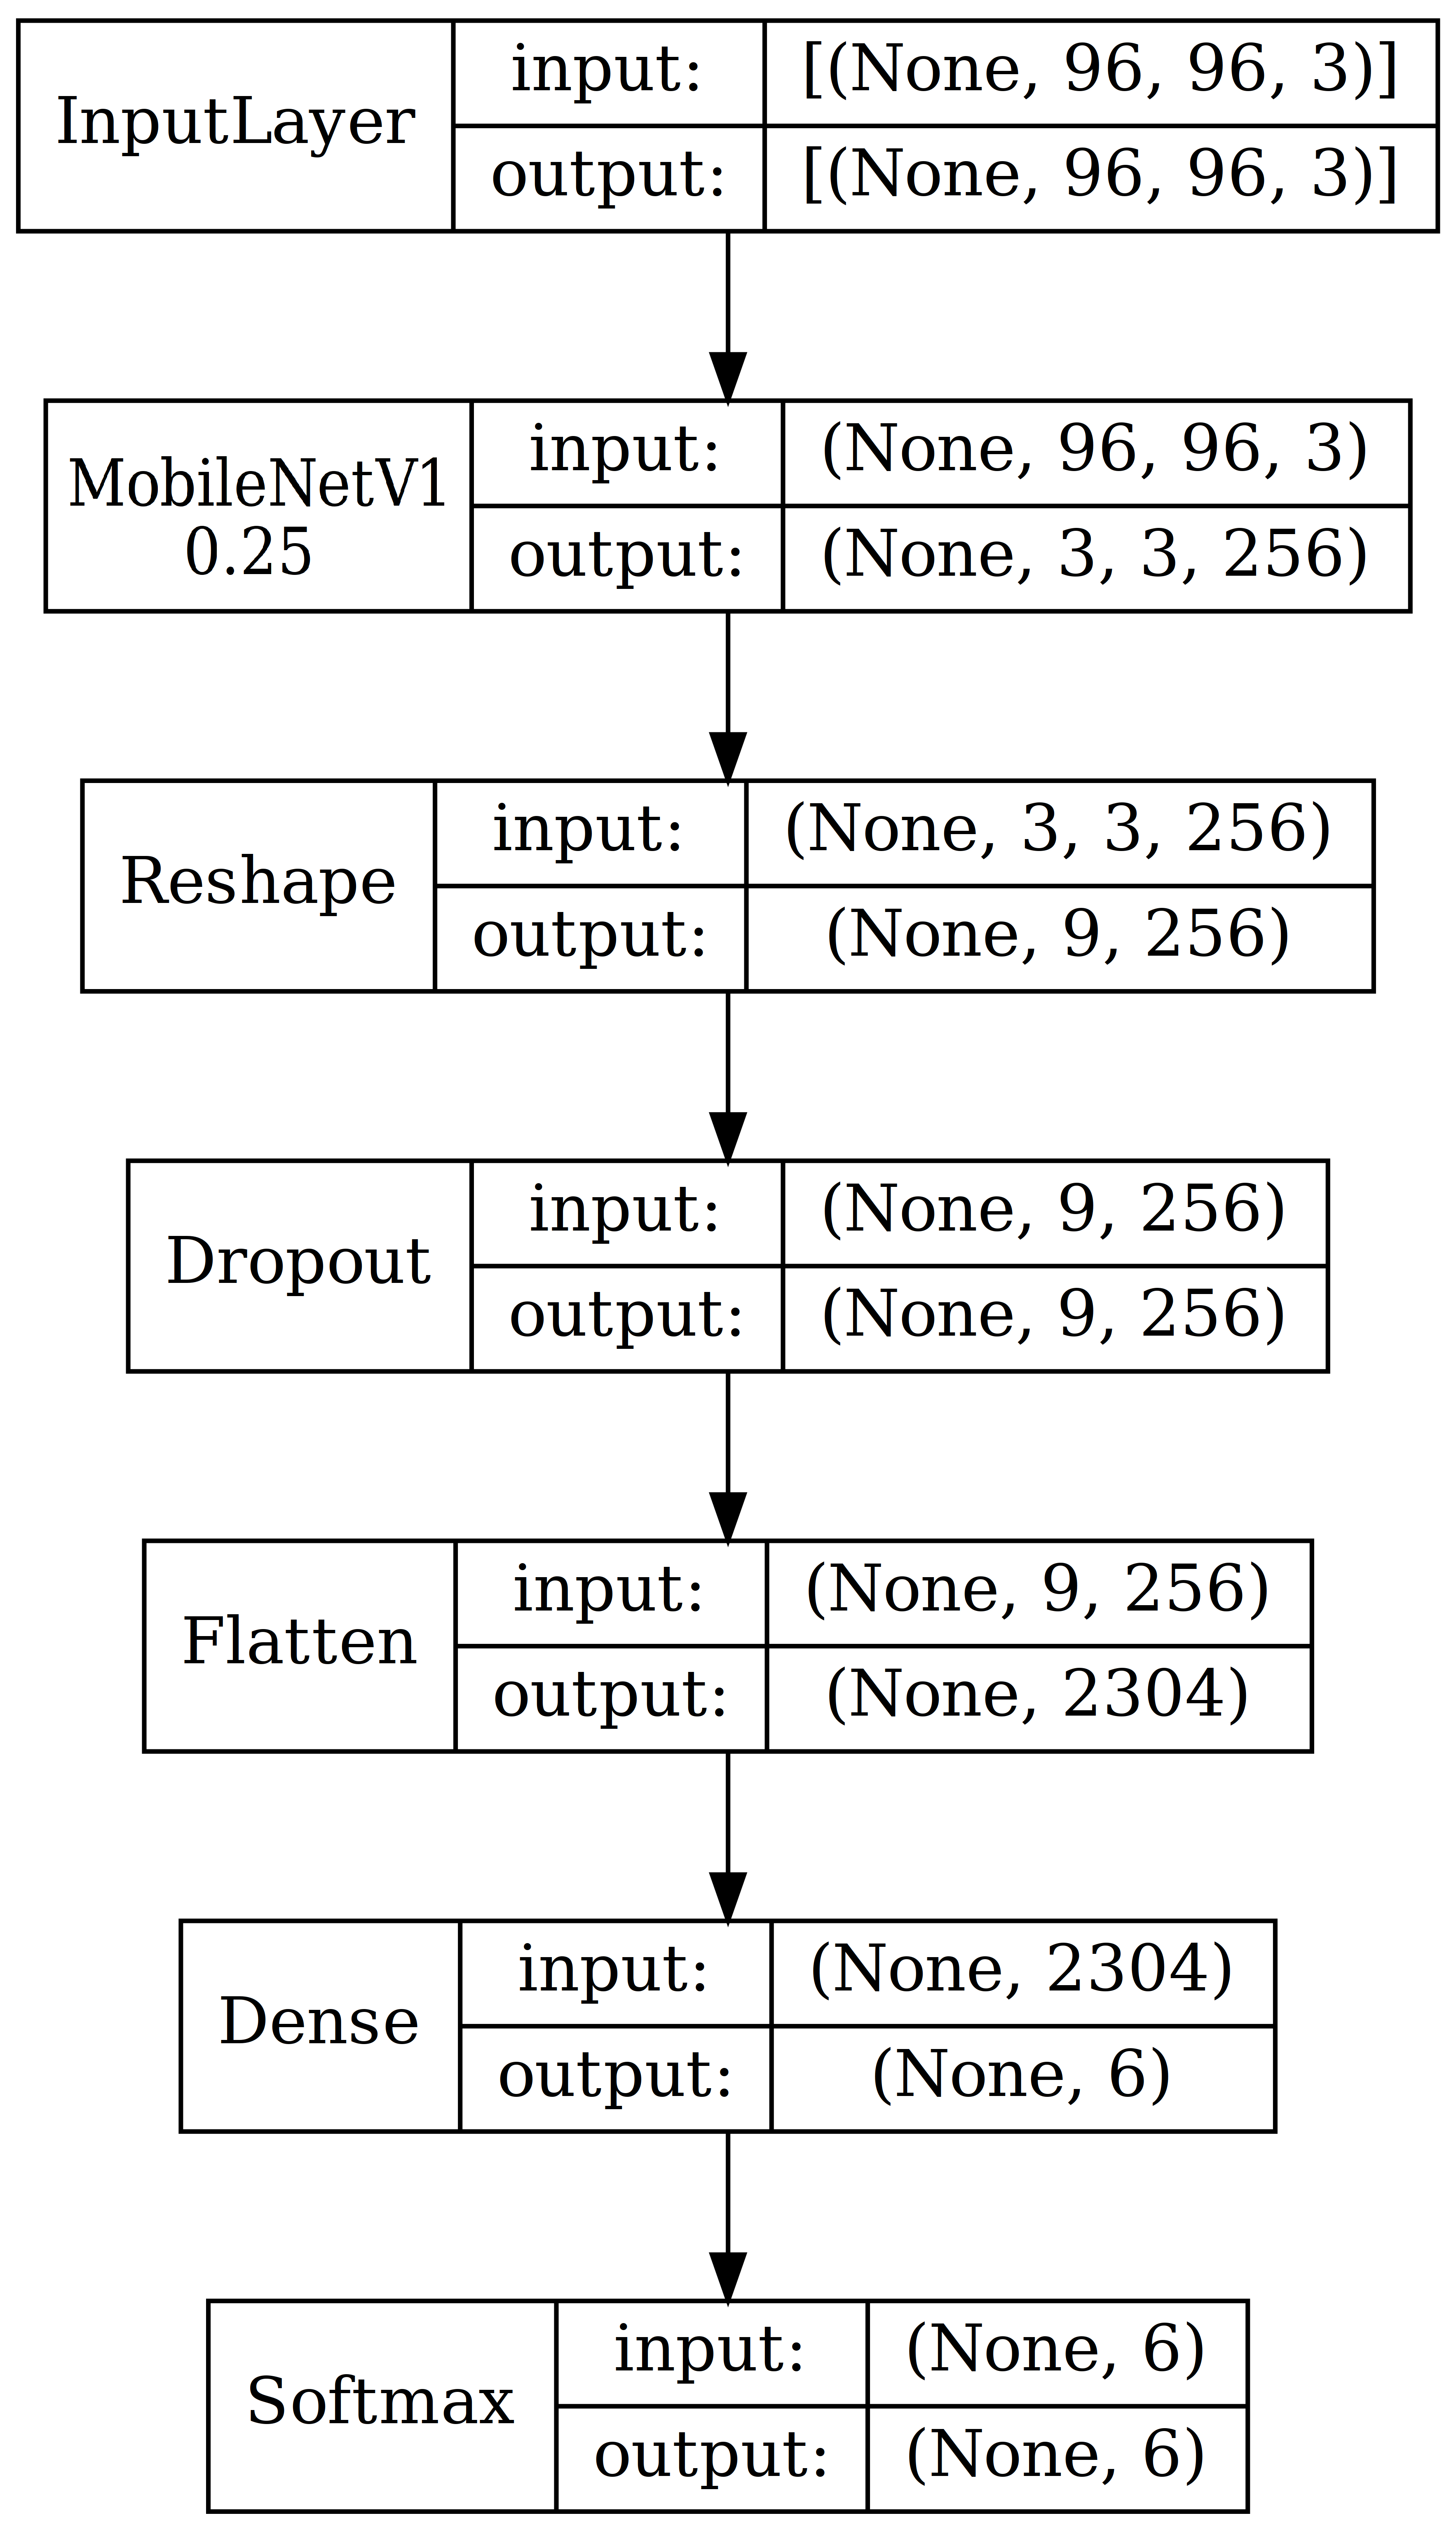
\includegraphics[width=0.35\textwidth]{Figures/5-gestures/5_model.png}
    \caption{The architecture of the \textit{5-gestures} model, with a focus on the layer type and on the input and output shapes.}
    \label{fig:5_architecture}
\end{figure}


\section{Model training}
\label{sec:5-training}
The training is also very similar: it is divided in the same way into two phases, the \textit{fit} phase and the \textit{fine-tuning} phase. 

In both steps, we are using the Adam optimizer and the Sparse Categorical Cross Entropy loss function in order to perform the gradient descent and the back-propagation. 

For the \textit{fit} phase, we are using an initial learning rate of $0.001$ and training for $20$ epochs. For the \textit{fine-tuning} phase, we are using a much smaller learning rate of $0.00001$ in order to avoid the phenomenon called catastrophic forgetting on the weights of the base model, and training for $20$ epochs.

The final results of the training, i.e. the results of the \textit{fine-tuning} phase, are displayed in the following charts.

\begin{figure}[H]
  \centering
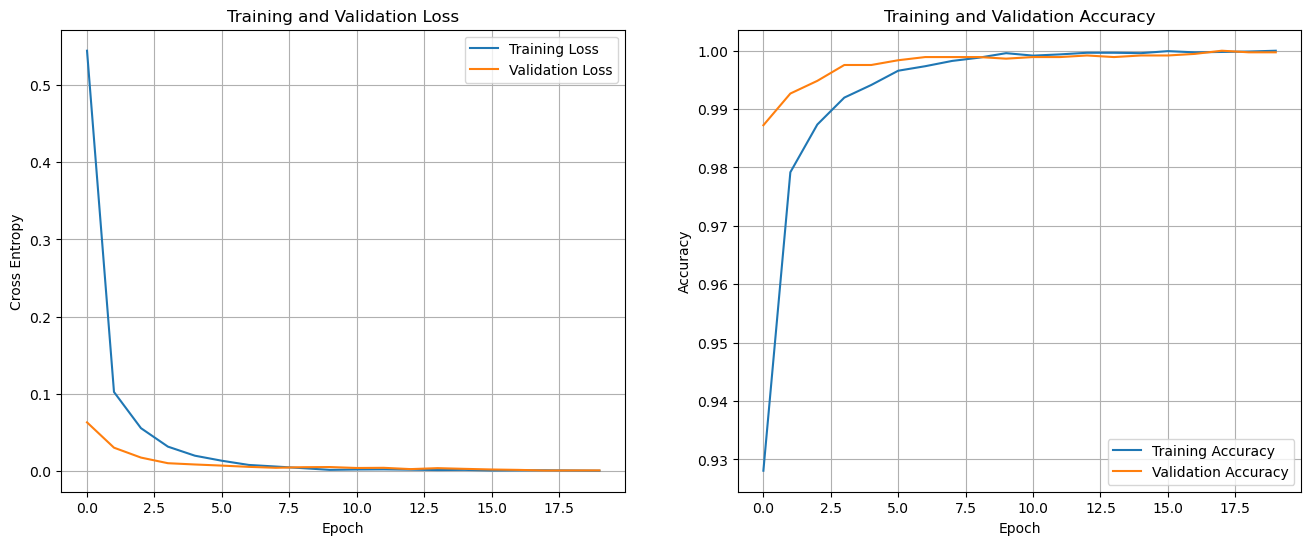
\includegraphics[width=\textwidth]{Figures/5-gestures/5_loss.png}
\caption{Evolution of the loss function and of the accuracy of the \textit{5-gestures} model on both the training and the validation sets.}
\label{fig:5_loss}
\end{figure}


\section{Model evaluation}
\label{sec:5-evaluation}
From Figure \ref{fig:5_loss} we can see that the model reached the highest accuracy possible, as expected since it was already achieving an excellent accuracy in the original 29-classes problem which was more complex.

In the following chart, we report a confusion matrix that represents the performance of the on a per-class basis.

\begin{figure}[H]
   \centering
   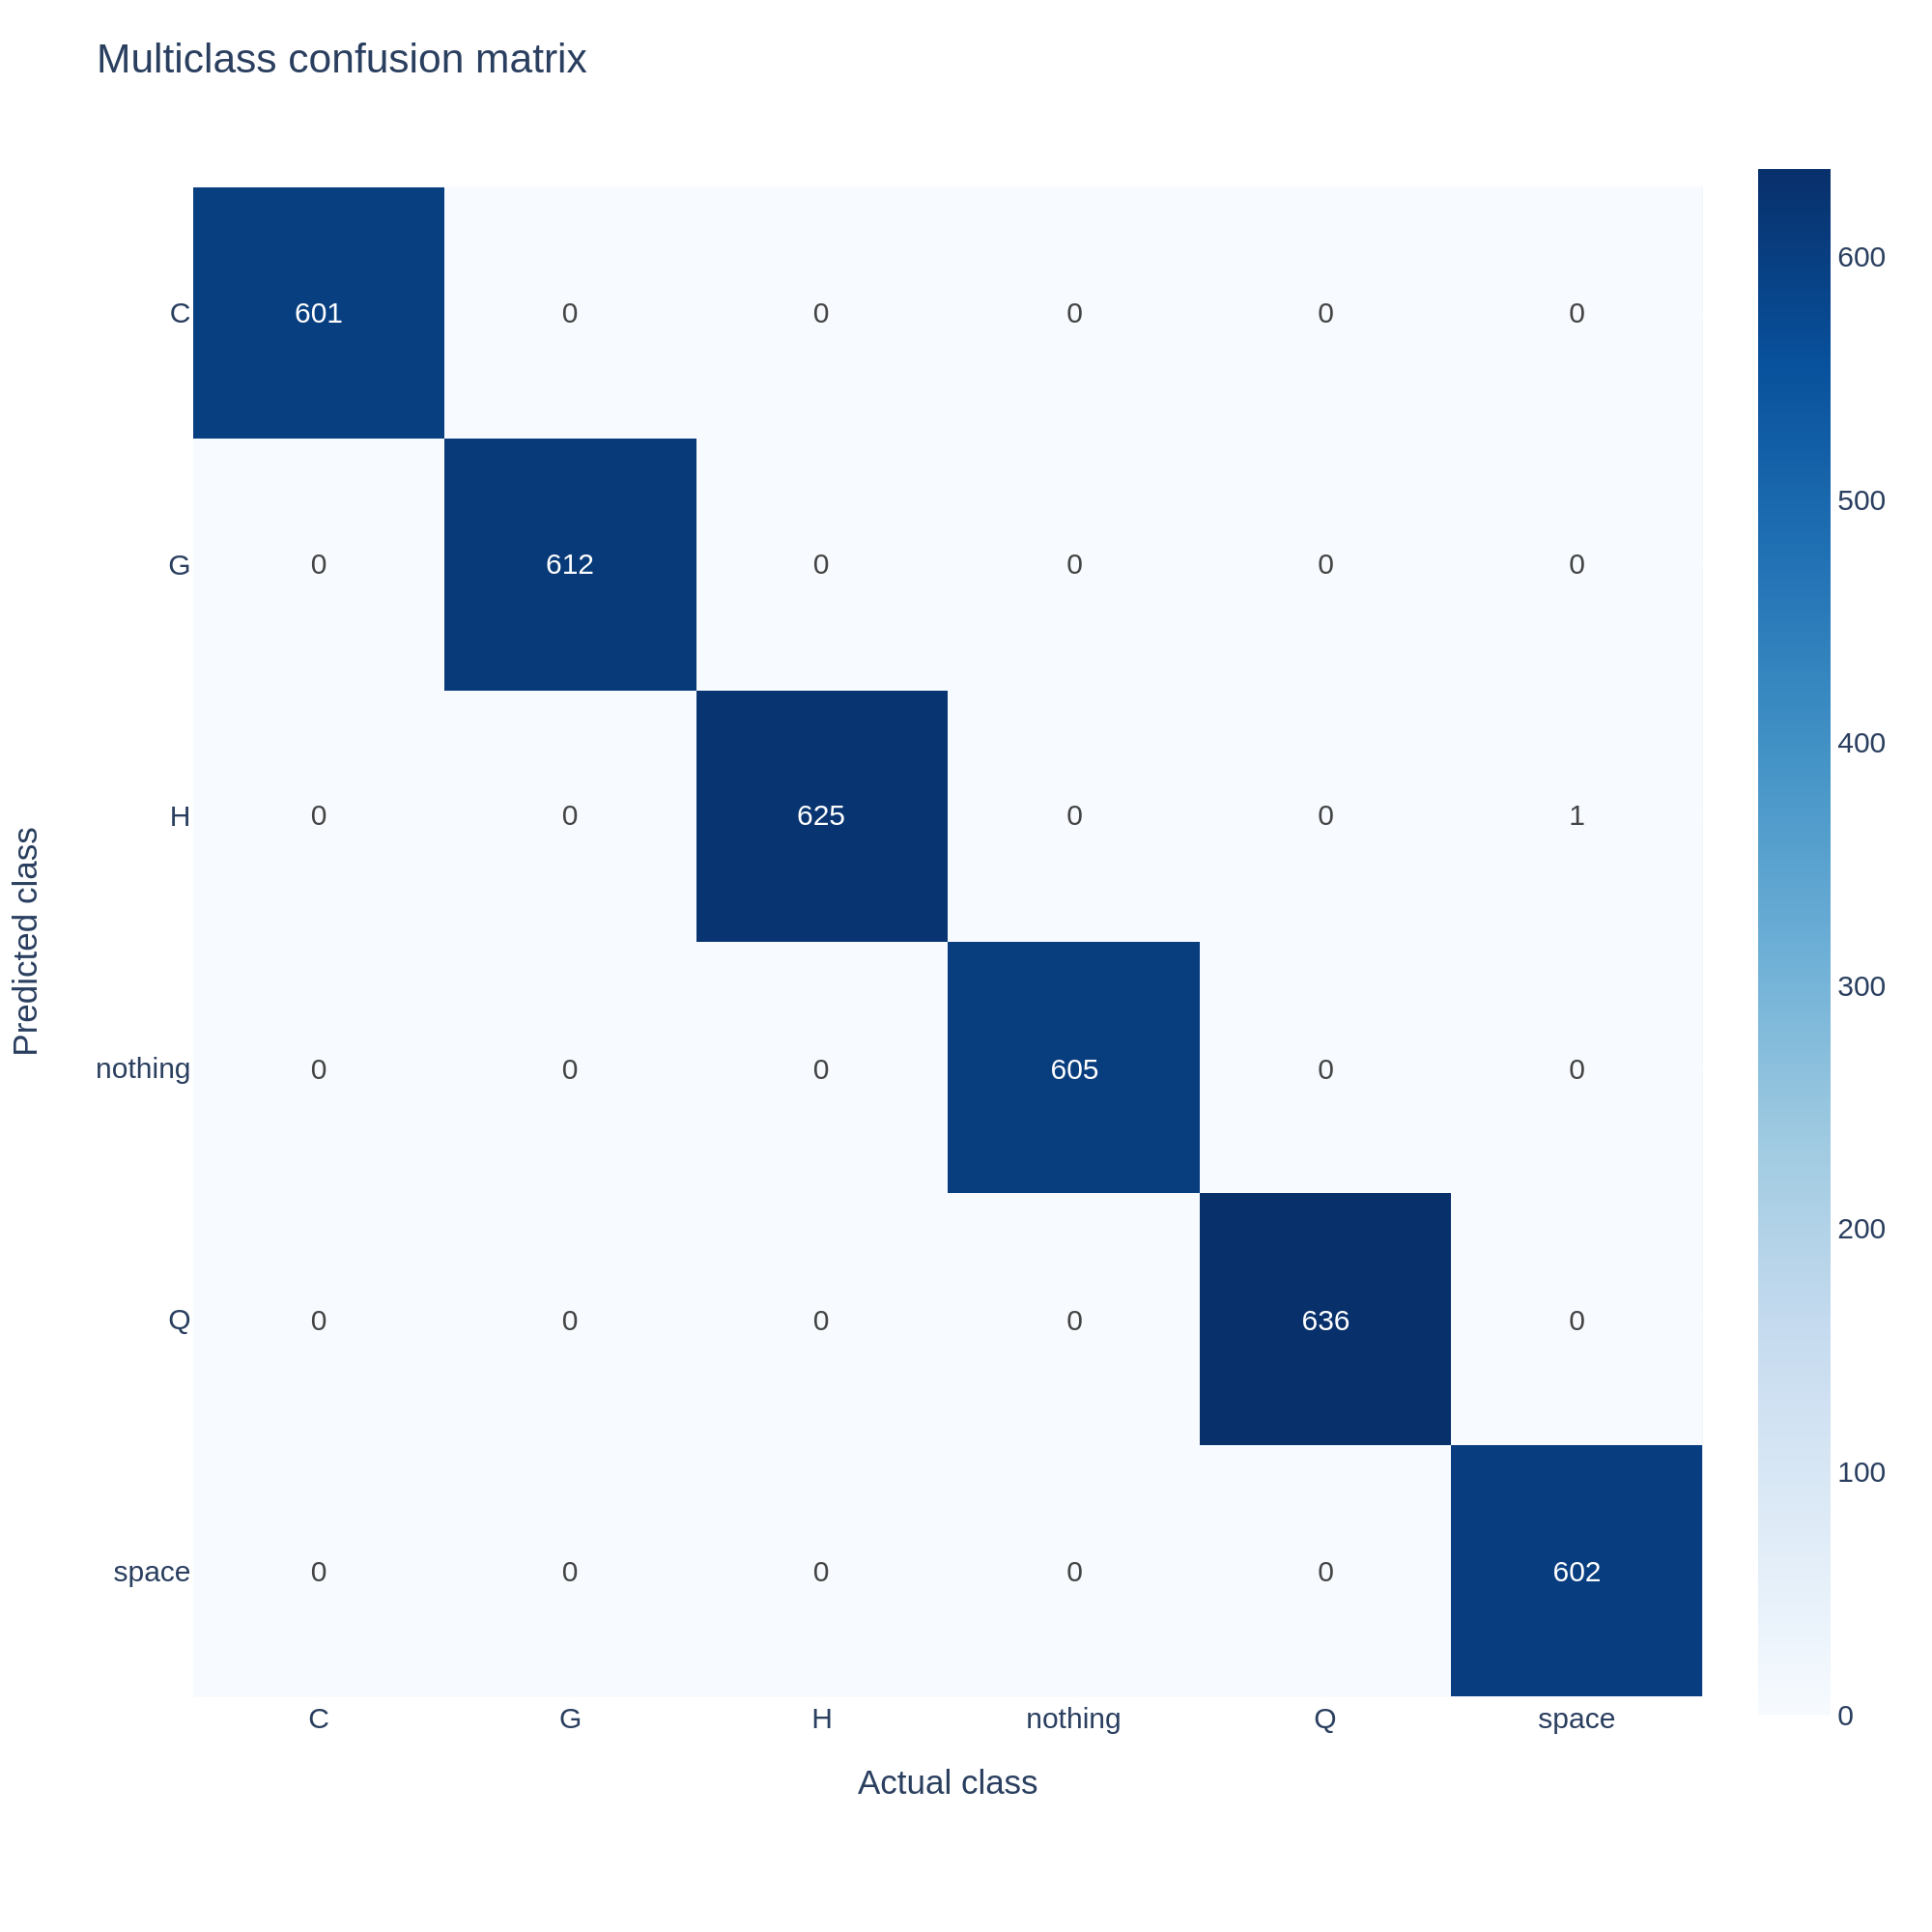
\includegraphics[width=0.7\textwidth]{Figures/5-gestures/5_cm.png}
   \caption{Confusion matrix on the validation set of the \textit{5-gestures} model.}
   \label{fig:5_cmatrix}
\end{figure}

In the following charts, we can instead see the normalized error counts per class of samples that the model fails to classify correctly, for each class.

\begin{figure}[H]
   \centering
   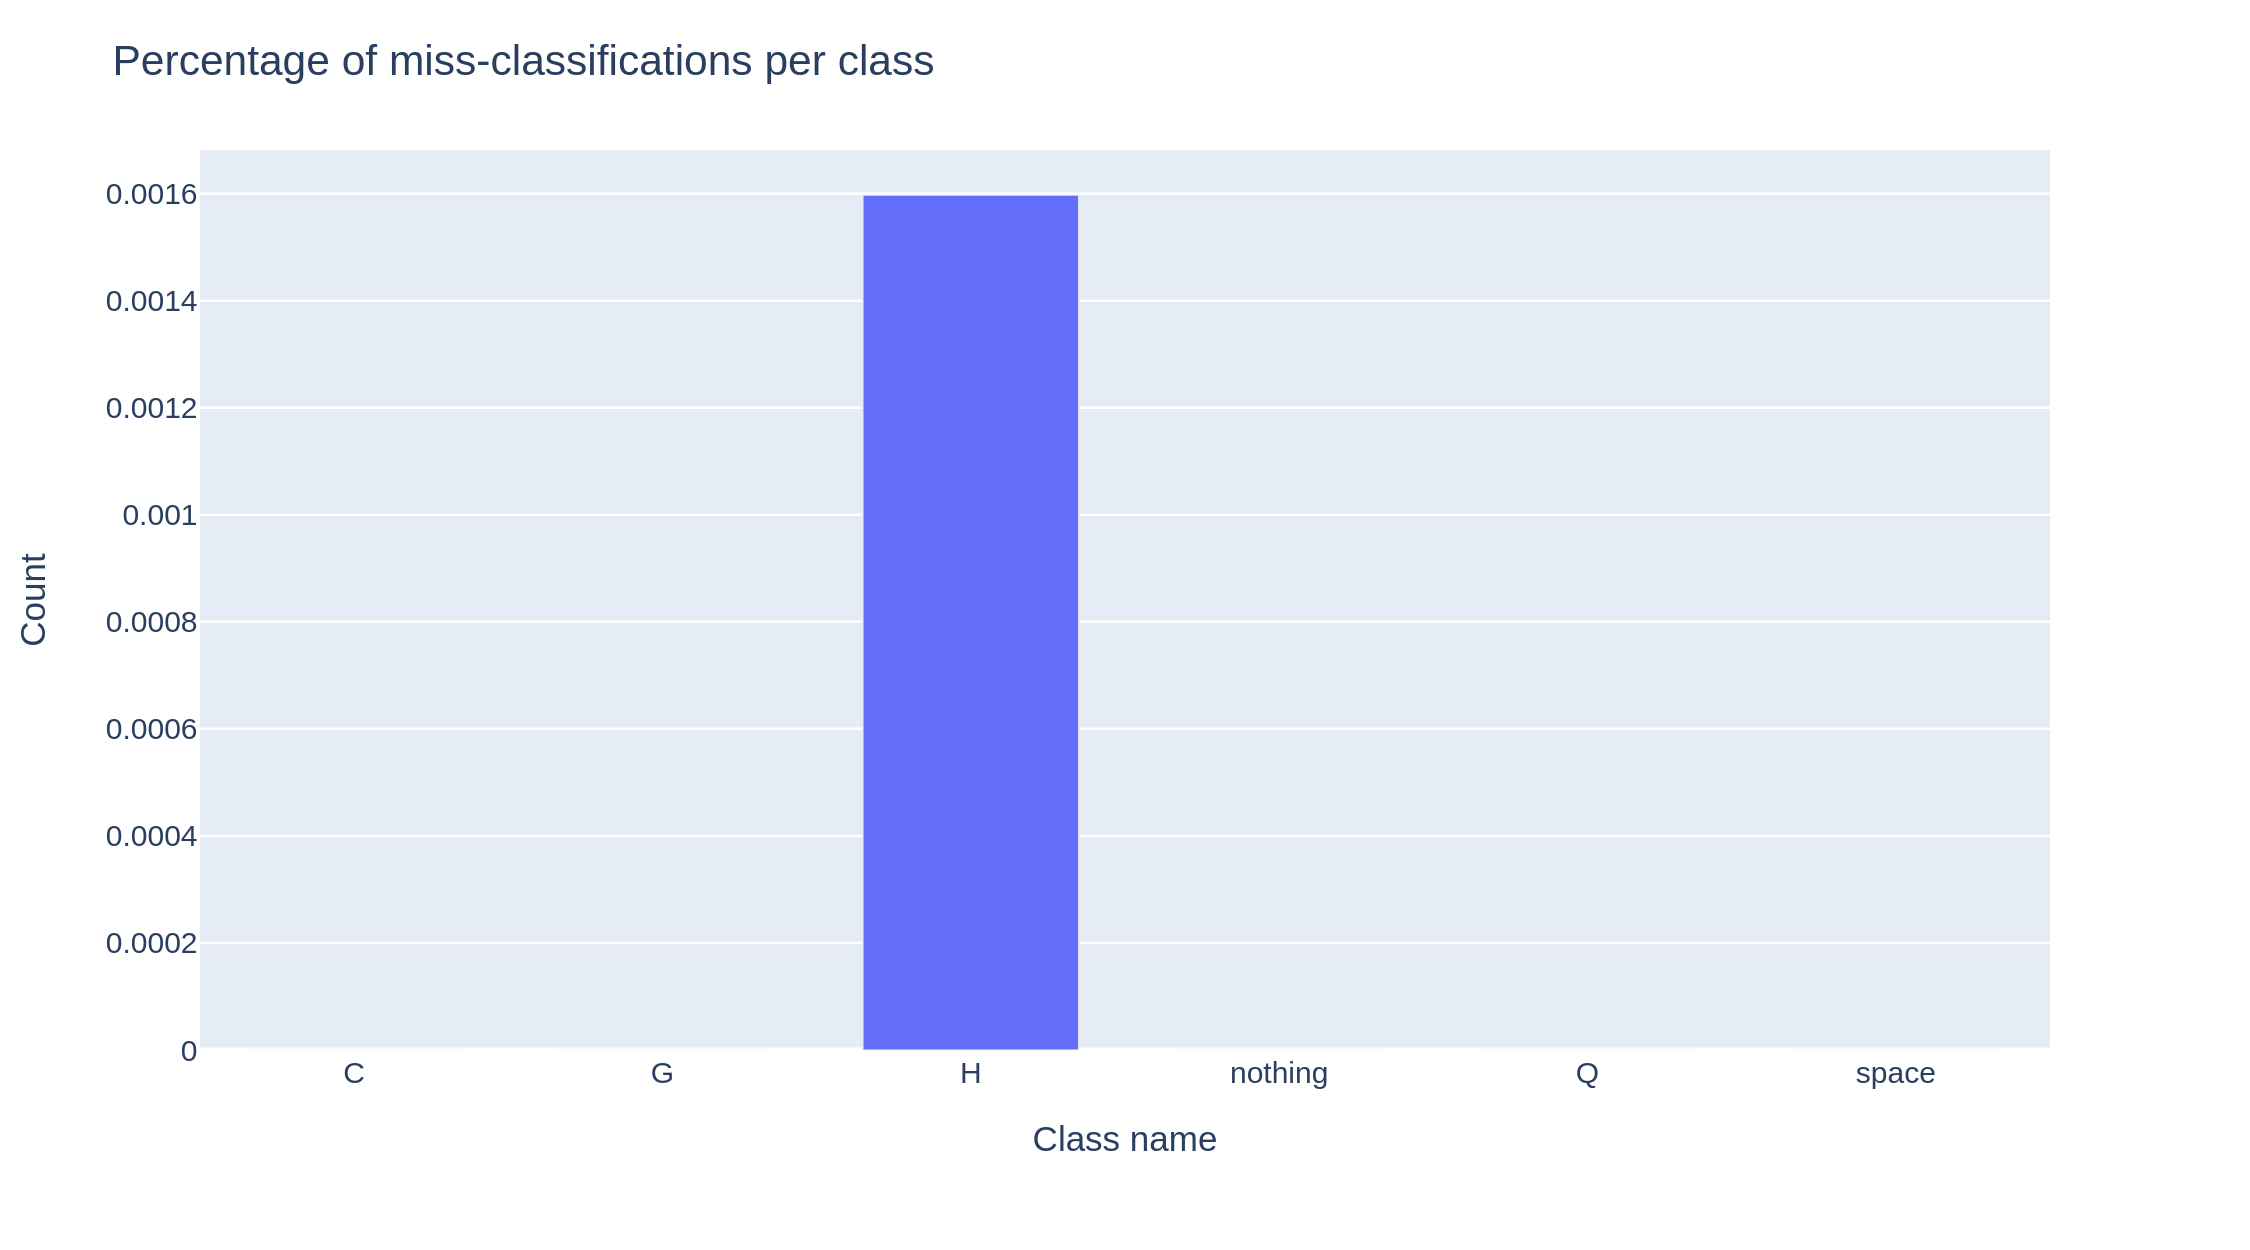
\includegraphics[width=0.85\textwidth]{Figures/5-gestures/5_errors.png}
   \caption{Percentage of miss-classification per class of the \textit{5-gestures} model.}
   \label{fig:5_errors}
\end{figure}

We can see that the performance of the model is excellent. Therefore, we are ready to perform the next step, which is quantizing the model in order to reduce its memory occupation. Without this step, the model would be too large to fit on the device. Quantization is covered in the next chapter.


\chapter{Quantization}
\label{ch:quantization}%
The aim of the quantization step is to transform a 32-bit floating point model, into a smaller 8-bit model, in order to make it deployable on our Arduino device, which as already mentioned features a very small amount of memory only. This step allows also for minimizing the inference time, the dimension of the model, and the average RAM usage during the inference time, while the performance of the model can remain approximately the same.

The quantization step has initially been performed by applying Post Training Quantization (PTQ), which takes the non-quantized TensorFlow model and commutes it into a quantized TensorFlow Lite model. In order to obtain the best model possible, we generated 3 different models with 3 different "levels" of quantization.

N.B: The metric of "better" is defined not only by the accuracy but also by the time and memory demand requested during the inference and by the model dimension.

Types of quantizations: 
\begin{enumerate}
    \item \textbf{Not quantized:} this model has just been converted into a TFLite model deployable on the Arduino, without optimizations.
    \item \textbf{Dynamic Range Quantization:} the weights of this model have been statically quantized from floating point to integer at conversion time, which provides 8 bits of precision. However, the outputs of the feature maps are still stored using floating point.
    \item \textbf{Full Integer Quantization:} the weights have been quantized dynamically to 8 bits of precision using a representative dataset. This version enforces quantization for all operations. 
\end{enumerate}
 
\begin{table}[H]
    \centering 
    \begin{tabular}{|p{15em} c c c |}
    \hline
    \rowcolor{bluepoli!40}
     \textbf{Quantization type} & \textbf{Size [KB]} & \textbf{Latency [it/s]} & \textbf{Accuracy} \T\B \\
    \hline \hline
    \textbf{No quantization} & 895.00 & 79.11 & 0.999 \T\B \\
    \textbf{Dynamic Range quantization} & 283.90 & 56.10 & 0.998\T\B\\
    \textbf{Full integer quantization} & 313.27 & 59.98 & 0.991 \B\\
    \hline
    \end{tabular}
    \\[10pt]
    \caption{Statistics of the model after different kinds of quantization have been applied.}
    \label{table:quantization_results}
\end{table}


We can notice from the table above that the model with the best overall statistics is the second one. Ideally, we would choose that model, but given that the Microcontroller (MCU) of our target device supports only full integer models, we chose the third one as a final model. 

Consequently, we performed full integer quantization on the original TF model, which also converted it into a TFLite model. In the following charts, a confusion matrix of the predictions and the percentage of miss-classifications of the quantized model is shown.
\begin{figure}[H]
   \centering
   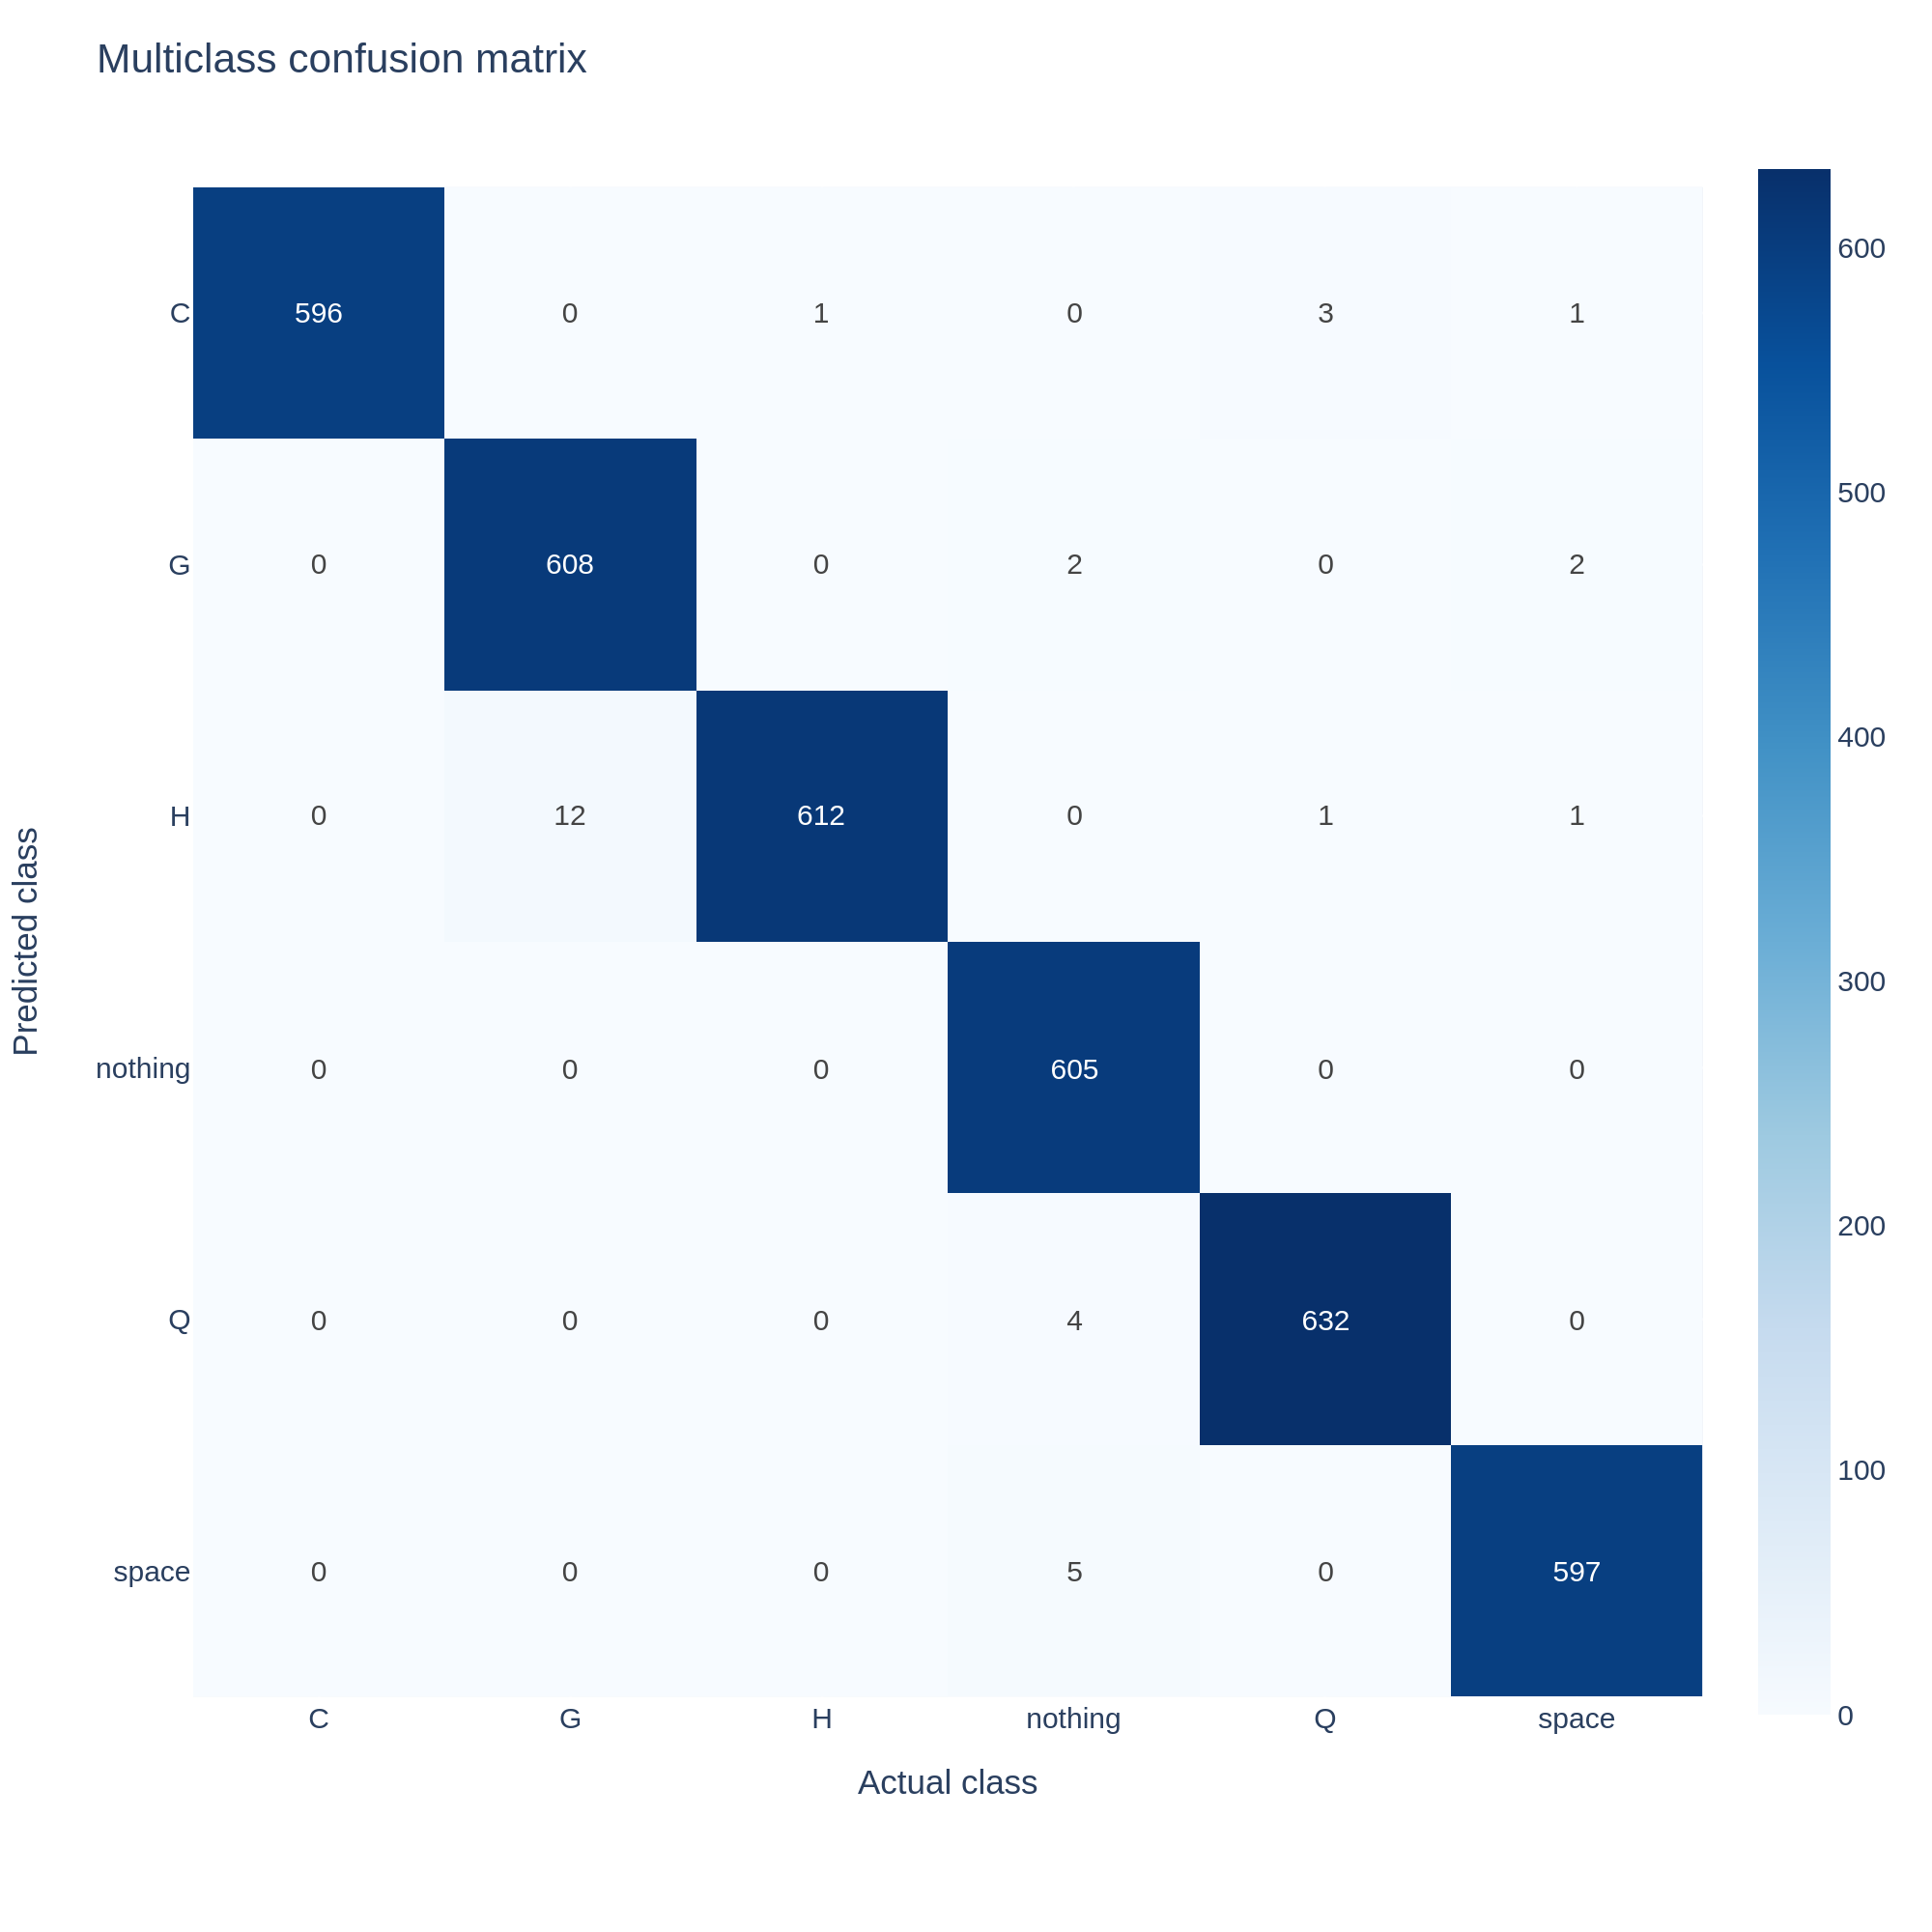
\includegraphics[width=0.6\textwidth]{Figures/5-gestures/5_cm_quant.png}
   \caption{Confusion matrix on the validation set of the quantized \textit{5-gestures} model.}
   \label{fig:5_cmatrix_quant}
\end{figure}

\begin{figure}[H]
   \centering
   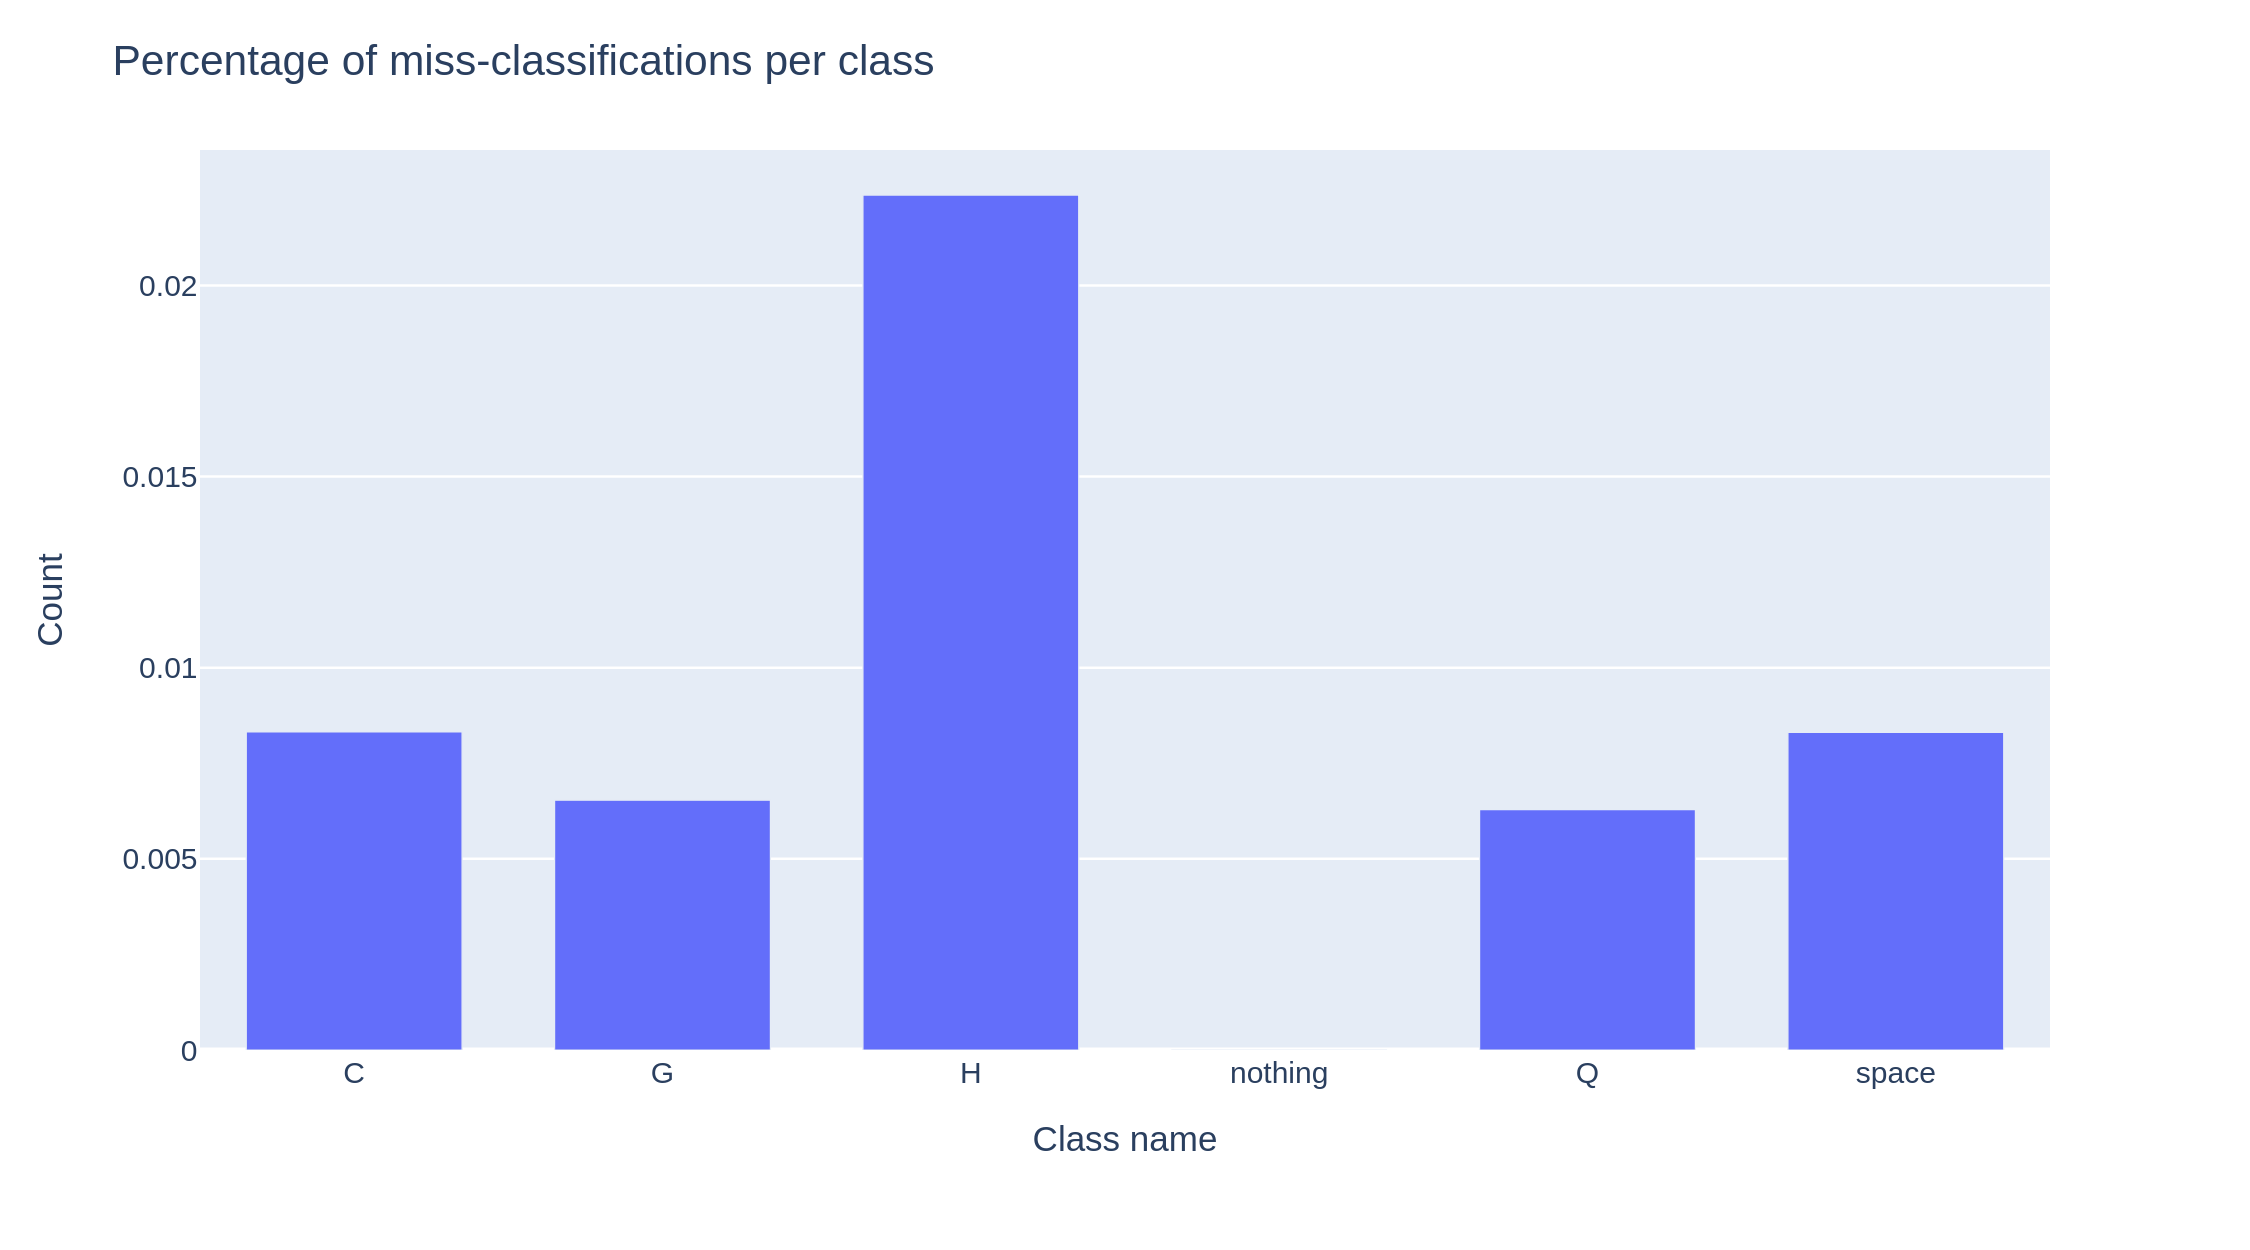
\includegraphics[width=0.8\textwidth]{Figures/5-gestures/5_quant_errors.png}
   \caption{Percentage of miss-classification per class of the quantized \textit{5-gestures} model.}
   \label{fig:5_errors_quant}
\end{figure}

We can see that as expected the quantized model performs slightly worse than the unoptimized one, but its accuracy is still very high nonetheless. We proceed to the deployment phase, in order to finally upload the model into the target device.


\chapter{Deployment}
\label{ch:deployment}%
The deployment phase involves transferring the neural network onto the physical device.
In order to do it, it's necessary to build the Arduino library and add it to the Arduino IDE libraries, so it will be possible to upload the network on the device and run it in the real world, using the Arduino Nano 33 BLE camera to take pictures and apply the inference.

To build the Arduino library, we uploaded the TFLite model we described in the previous chapter into Edge Impulse. Subsequently, Edge Impulse generated a library encapsulating both the model's weights and the necessary code for executing inference. 

However, we quickly realized that, although our model fit within the device's memory, there was insufficient space to accommodate the intermediate feature maps of the model. Consequently, conducting inference on the device was unfeasible.

As a solution, we retrained the identical model on the same dataset, opting to use Edge Impulse directly instead of TensorFlow. Edge Impulse also handled the quantization process, and the deployment was executed in a similar manner. This time, it was possible to use the model on-device to perform inference on real-world data. This suggests that Edge Impulse utilizes some additional optimizations to reduce the size of the model even further.


\section{Real-world performance}
\label{sec:real_word_perf}
After having deployed the \textit{5-gestures} model on the device, it was found that the accuracy was very poor. The project was tested for some time, with the hands of different individuals and using different backgrounds and lights, but the Arduino output was rarely correct. 

We attribute this issue largely to the limited variability in the dataset. Given that all samples were presumably collected by a single individual in a single room, the dataset lacked the necessary diversity. This led to a search for another, more diverse dataset. 

\chapter{Data collection}
\label{ch:data-coll}%
With the aim of enhancing the dataset, we looked for another dataset, with the hope of finding one created by multiple contributors with varied backgrounds.

Our search led us to the ASL Alphabet Test \cite{asl_test} dataset, which has 30 images for each class, for a total of 870 samples. The images are 256 x 256 8-bit photos to match the ASL Alphabet dataset. This dataset is much more variegate with very a large diversity of lighting conditions and backgrounds. 

Subsequently, we employed the OV7675 Camera interfaced with the Arduino to directly capture samples.
This step was possible thanks to Edge Impulse, which has a section that helps in collecting data directly from the device. It is sufficient to connect the device to the PC, establish a serial connection with Edge Impulse, and select the sensor we want. It will be possible to see the live camera output and take pictures by clicking a button; the collected image can be labeled with the class we want and added to the dataset.
This process was applied in order to collect real-world data, with different types of background/light and different people's hands, so the dataset could be as general as possible.

\begin{figure}[H]
    \centering
    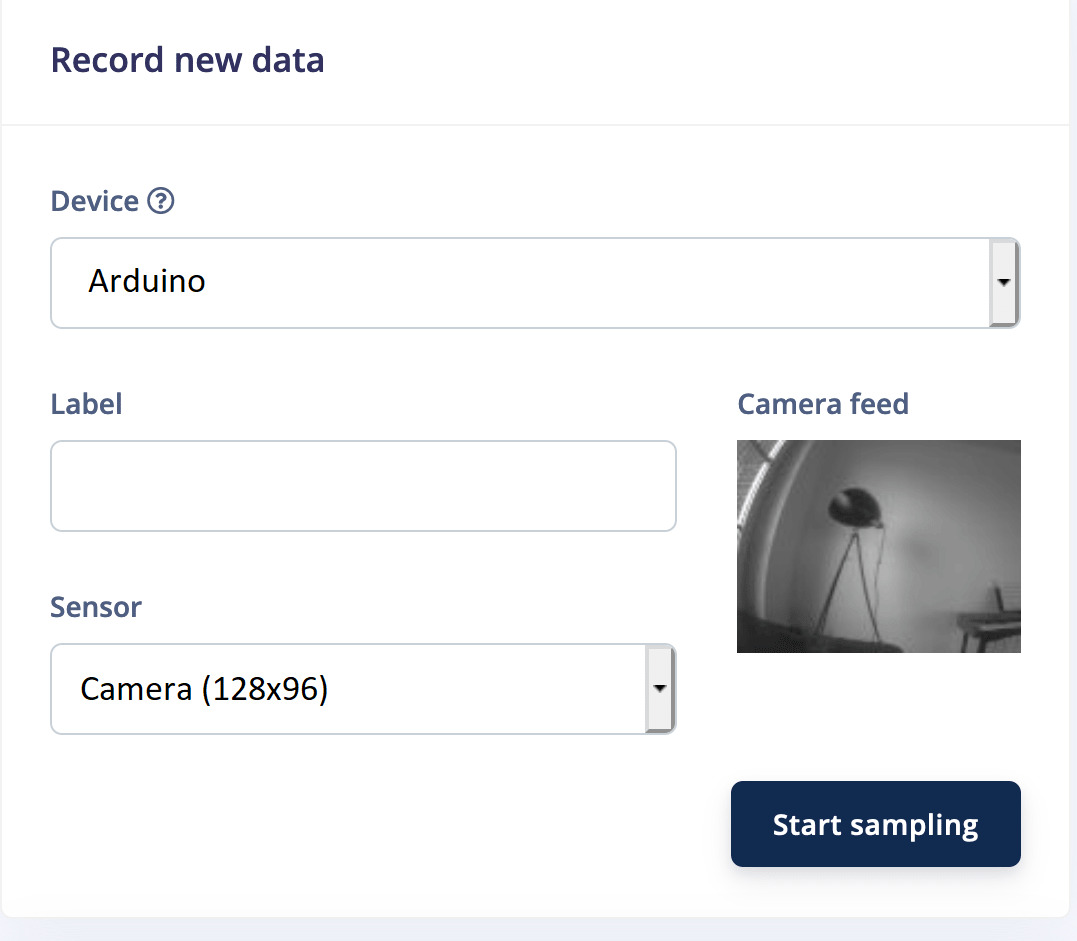
\includegraphics[width=0.5\linewidth]{camera-feeed.jpg}
    \caption{Edge Impulse data collection tool}
    \label{fig:data-collection}
\end{figure}

From this moment on, we will refer to the 3 datasets we are working with using the following nomenclature:
\begin{itemize}
    \item \textit{ASL Classic}: the original dataset we started our work with
    \item \textit{ASL Real}: the ASL Alphabet Test introduced at the beginning of this section
    \item \textit{ASL Device}: the dataset we personally collected using the Camera of the device
\end{itemize}

We merged the 3 datasets into one, which we called \textit{ASL Final} dataset. In order to introduce the least possible amount of bias in the new dataset, we decided to keep the distribution of the 3 separate datasets equal: for each gesture, we introduced 30 (which is the number of samples of the \textit{ASL Real} dataset) samples per dataset, resulting in a total of 90 samples per class. 
As a consequence, the ASL Final dataset encompasses 540 samples in total.
\begin{figure}[H]
    \centering
    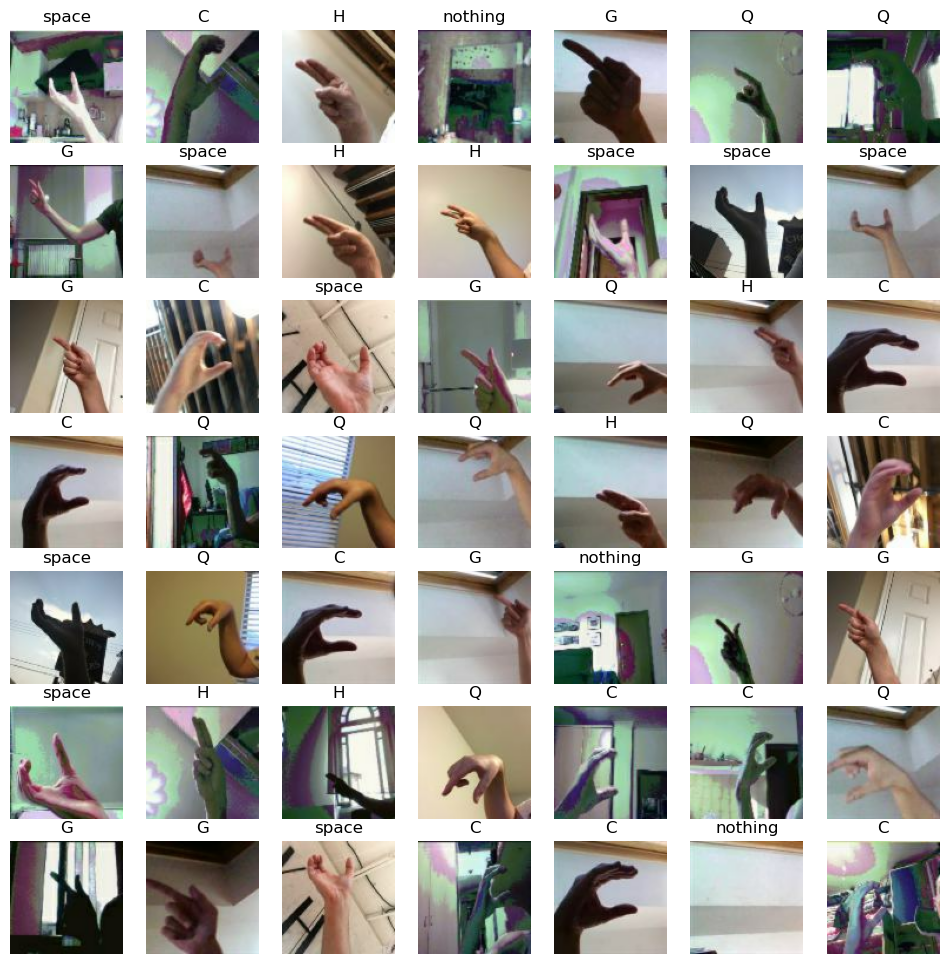
\includegraphics[width=0.8\textwidth]{Figures/asl_final_images.png}
    \caption{Visualization of 49 samples from the \textit{ASL Final} dataset}
    \label{fig:asl_final}
\end{figure}

Then, we decided to test the performance of the \textit{5-gestures} model on the new \textit{ASL Final} dataset. We divided the dataset into a train set composed of 80\% of the samples and a validation set composed of 20\% of the samples. This is to allow for a fair comparison with the model we are going to build later. This analysis can be found in the last section of the\textit{ 5-gestures model.ipynb} notebook of the GitHub repository. 

The accuracy of the \textit{5-gestures} model on the validation turned out to be 61.11\%. As expected, it is much lower than 99\%. Given that the \textit{5-gestures} model had already seen basically all samples from the \textit{ASL Classic} dataset during its training phase, we decided to test its performance first using samples coming from the \textit{ASL Real} dataset only and then with samples from the \textit{ASL Device} only. 

This further examination revealed that when tested exclusively on samples from the \textit{ASL Real }dataset, the model achieved an accuracy of 48.89\%. However, its performance dramatically declined to 29.44\% when assessed with samples from the \textit{ASL Device} dataset.

From these tests, it is clear that \textit{the 5-gestures} model overfitted the specific lighting conditions and backgrounds prevalent in the \textit{ASL Classic} dataset, and that was why it was performing so poorly when deployed in the real world.



\chapter{5-gestures-v2 Model }
\label{ch:5-v2-model}%
Now that we have a new, much more diverse dataset, we can finally train the last model, with the high hope that a good performance on our ensemble of datasets will translate into a good performance with real-world data. This model, built upon a more diverse dataset, showcases the potential to excel in practical applications and is referred to as \textit{5-gestures-v2} model. 

This analysis was performed by using both TensorFlow and Edge Impulse. TensorFlow was used in our local machine in order to experiment faster with the model architecture and hyperparameters. Once the best architecture was found, the model was trained and then deployed using Edge Impulse. The source code can be found in the notebook \textit{5-gestures-v2 model.ipynb} of the GitHub repository. 


\section{Model architecture}
\label{sec:5-v2-arch}
The architecture of this model is the same as the \textit{5-gestures} model (refer to Figure \ref{fig:5_architecture}). However, this time we have at our disposal a much, much smaller amount of data since our dataset consists of only 90 samples per class. Normally, this amount of samples is insufficient to effectively train a Deep Learning model. However, we trust they will be enough for our specific setting, thanks to the following factors:
\begin{itemize}
    \item The model we are working with is tiny and therefore less prone to overfitting
    \item We are using Transfer Learning, which is known to work well even with very little data to learn from
    \item We can counter overfitting by tweaking the dropout rate of the Dropout layers inside both the \textit{base} model (MobileNetV1) and the dense classifier. A higher dropout rate will force the model to generalize better, therefore reducing overfitting
    \item We can use data augmentation techniques in order to artificially expand the training dataset, providing the model with more diverse examples to learn from
    \item We are not aiming for \textit{perfect} accuracy: due to the diversity of this new dataset, the \textit{5-gestures-v2} model, even with a respectable accuracy (e.g., 70\%), is expected to outperform the \textit{5-gestures} model with 99\% accuracy in real-world scenarios
\end{itemize}

Following a phase of hyperparameter tuning, we ended up using the default dropout rate ($0.001$) for the base model and a dropout rate of $0.35$ in the dense classifier. Furthermore, we used the following data augmentation techniques, manually editing the default data augmentation pipeline that Edge Impulse offers through to its \textit{Keras advanced mode}:
\begin{itemize}
    \item RandomCrop
    \item RandomBrigthness
    \item RandomContrast
    \item RandomSaturation
    \item RandomHue
\end{itemize}

It is worth noting that we refrained from applying common techniques like RandomRotation and RandomFlip since they would sometimes alter the original image by too much, potentially turning a gesture into another. 

Of particular note, the RandomHue technique, which adjusts the hue of the input RGB images by rotating the hue channel, proved exceptionally useful in our case since we observed that the OV7675 Camera tends to skew the colors of the image under sub-optimal lighting conditions, applying a greenish tint to a significant portion of the image. We are confident that this augmentation technique will allow the model to learn from and accurately classify such scenarios.


\section{Model training}
\label{sec:5-v2-training}
In this case, during training, only the \textit{fit} phase was executed, omitting the\textit{ fine-tuning} phase entirely. This is because experimental tests showed that performing the \textit{fine-tuning} phase had no positive effect on the performance of the model, and in fact also lowered it in some cases. This outcome is likely attributed to the constrained size of the dataset, which is enough to train the dense classifier part of the model but insufficient to train the whole base model, which is much larger. 

In the \textit{fit} phase, we are using the Adam optimizer and the Sparse Categorical Cross Entropy loss function in order to perform the gradient descent and the back-propagation. We are using an initial learning rate of $0.001$ and training for $100$ epochs.

The final results of the training, i.e. the results of the \textit{fit} phase, are displayed in the following charts.

\begin{figure}[H]
  \centering
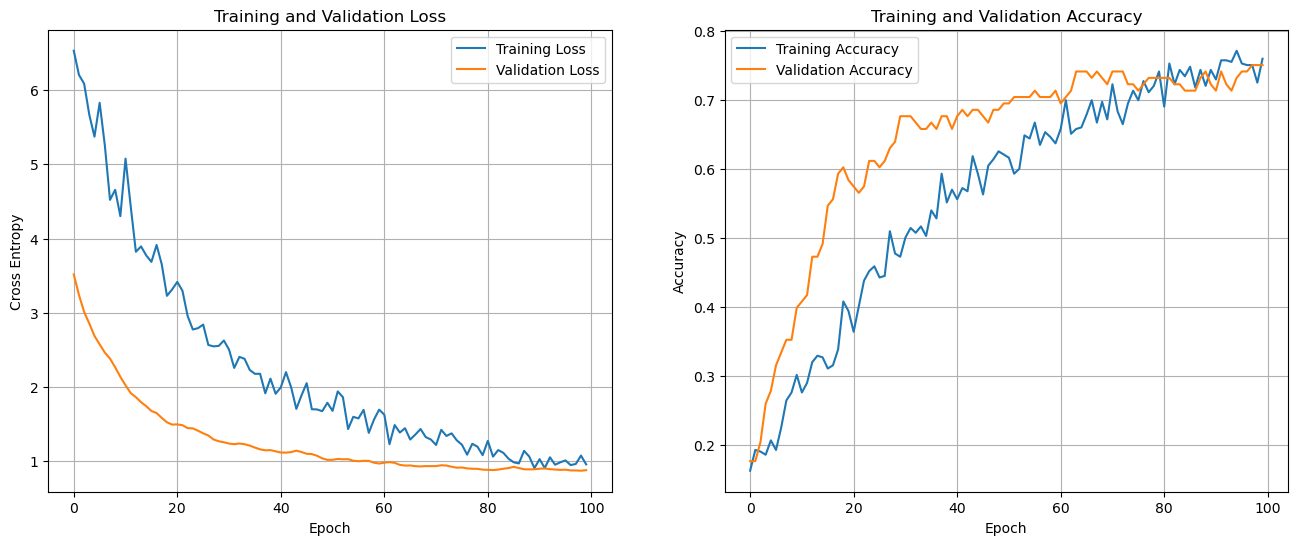
\includegraphics[width=\textwidth]{Figures/5-gestures-v2/5_v2_loss.png}
\caption{Evolution of the loss function and of the accuracy of the \textit{5-gestures-v2} model on both the training and the validation sets.}
\label{fig:5_v2_loss}
\end{figure}

As depicted in the above figure, the chosen hyperparameter configuration effectively mitigated overfitting, despite the restricted sample size at our disposal.


\section{Model evaluation}
\label{sec:5-v2-evaluation}
In this section, we take a closer look at the performance of the trained model. This time the training phase was conducted using Edge Impulse. In the figure below we can see a confusion matrix of the predictions of the (not yet quantized) model.

\begin{figure}[H]
   \centering
   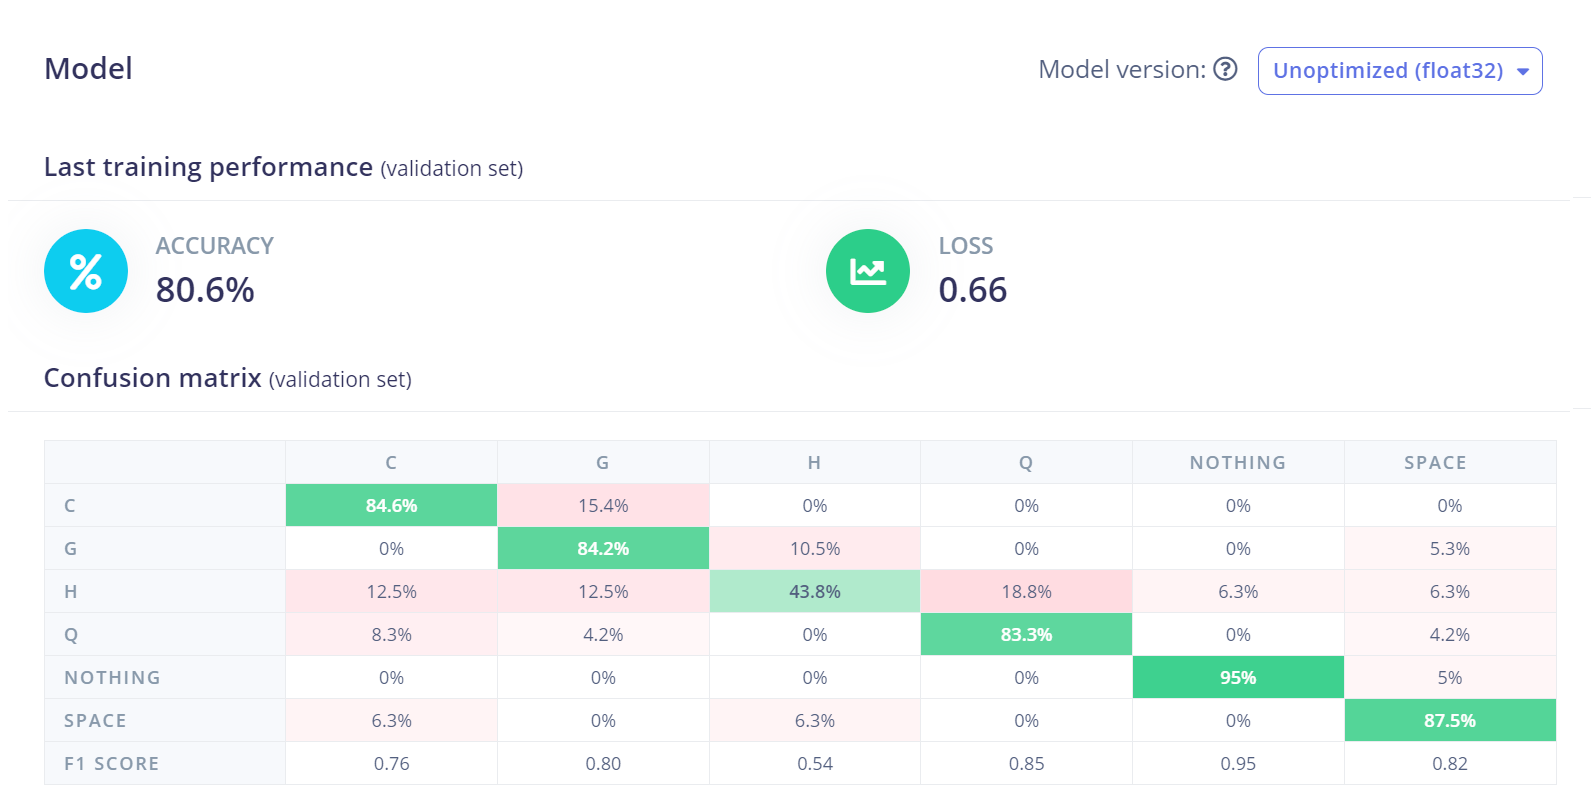
\includegraphics[width=0.85\textwidth]{Figures/5-gestures-v2/ei_v2_unoptimized.png}
   \caption{Confusion matrix on the unoptimized 32-bit \textit{5-gestures-v2} model.}
   \label{fig:5_v2_cmatrix_unoptim}
\end{figure}

The model was also able to reach a commendable accuracy of about $80$\%. Therefore, we expect that this model will perform well when deployed to the device.


\section{Quantization}
\label{sec:5-v2-quant}
The floating point model has been quantized directly on Edge Impulse, performing full integer quantization. In the figure below we can see a confusion matrix of the predictions of the quantized model.

\begin{figure}[H]
   \centering
   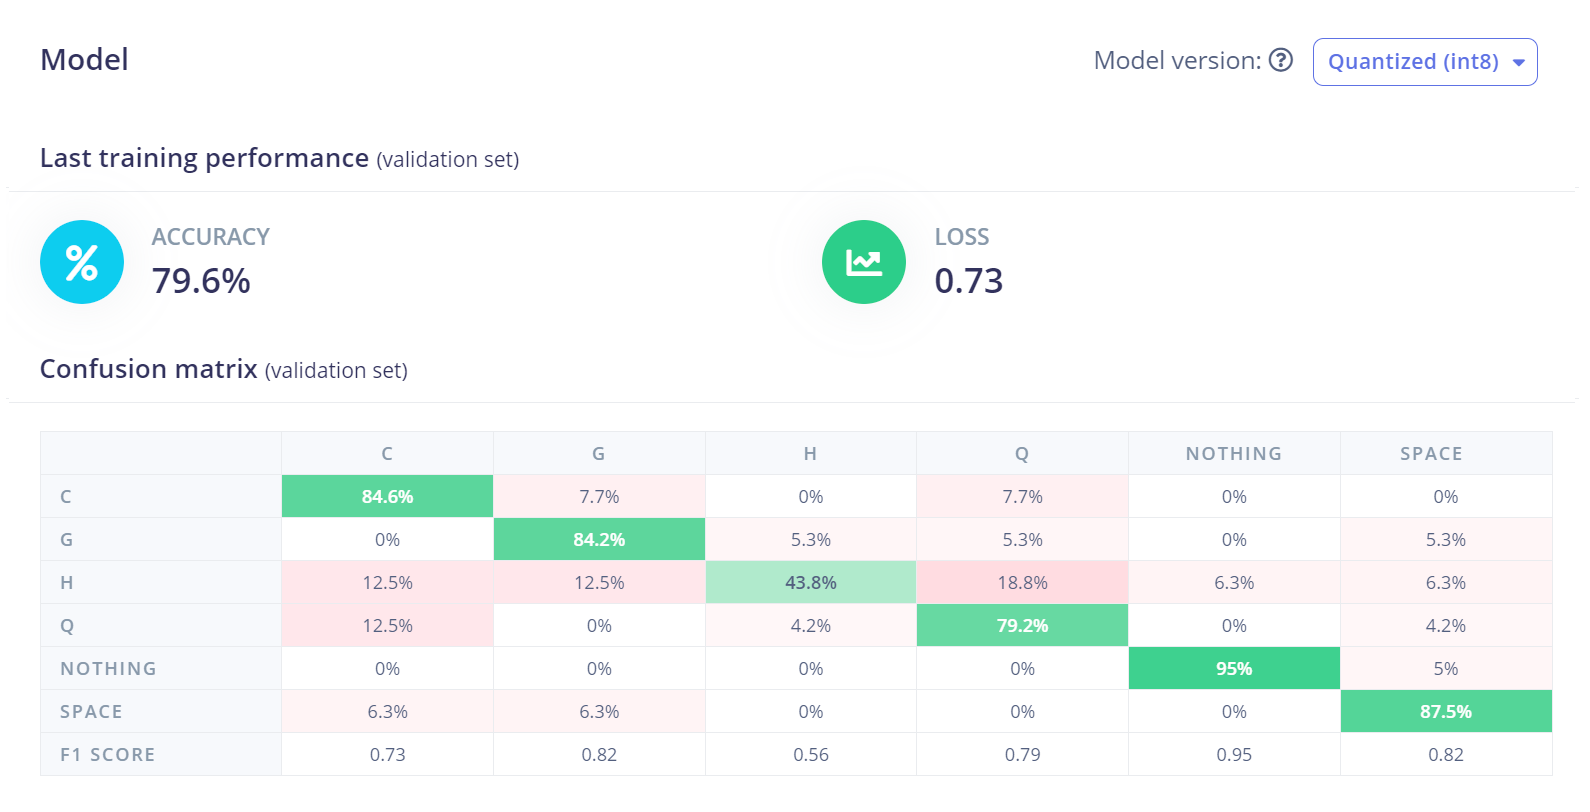
\includegraphics[width=0.85\textwidth]{Figures/5-gestures-v2/ei_v2_quant.png}
   \caption{Confusion matrix on the quantized \textit{5-gestures-v2} model.}
   \label{fig:5_v2_cmatrix_quant}
\end{figure}

It is evident that the difference in performance w.r.t. the unoptimized version is negligible. 


\section{Deployment}
\label{sec:5-v2-deployment}
In order to perform the deployment step, an Arduino library has been built, directly from Edge Impulse. Then, the library was added to Arduino IDE, and the "camera" example of that library was run on the device.

After being sure that the code was running and well working, some minor changes were made to the code, in particular, these changes were made in order to make a prediction valid only if its corresponding confidence is larger than $0.5$.

This step was implemented in order to minimize the output error of the project. The value 0.5, was found after several tests, and this was found out being the best value so far.


\chapter{On-device demo}
\label{ch:demo}%
In order to run the project, it is sufficient to upload the code on the device, being sure to place the device with its camera facing up, and, by selecting the correct serial port and opening the serial monitor, it will be possible to see the output of the device.

It will be visible as an official output, so it is the result that the device is giving, followed by the list of possible outputs coupled with their confidence.

\begin{figure}[H]
    \centering
    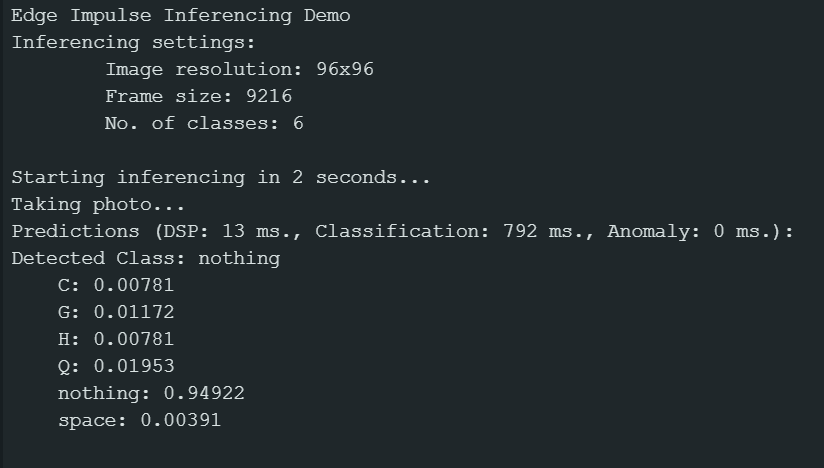
\includegraphics[width=1\linewidth]{inferencing img.png}
    \caption{Serial monitor showing Arduino output}
    \label{fig:demo}
\end{figure}


\chapter{Market}
\label{ch:market}%
This project could be used in several market fields, in fact, the purpose of this project would be to easily control some kind of device, by using hand gestures, just by connecting them together.

For example, this project could control a television, allowing the user to turn it on/off, change the channel, and raise or lower the volume, just by making smooth moves with their hand.

It could be also connected to a PC/smartphone webcam, so the user could set some fast frequent actions that the user is used to doing, in order to perform them just by a hand gesture, for instance, such as taking an actual picture that will be saved in the gallery, but also starting a program/app too.

Another application could be gesture recognition on a car during driving, allowing the driver to do fast, actions so that the driver doesn't have to be distracted while driving and is safer.

This project has been thought mostly for a consumer market.

\chapter{Ethics}
\label{ch:ethics}%
An important part of project development is the ethical implications: the developers must ensure to the users that their data will not be stolen or sold to anyone, and basically that the whole application is safe from an ethical perspective.

In particular, this project is ethical since:
\begin{itemize}
    \item Code, model, and training data are freely available (open-source) in the project repository
    \item At inference time, the data captured by the device is not stored or sent anywhere, but locally processed and deleted immediately after
    \item The model is not custom but the same for every user (therefore, even if you steal the device you cannot extrapolate information about the user from the model)
    \item The device is constantly monitoring the user when turned on, but this is not an issue since the data is not stored anywhere and the device is not transmitting it (e.g. through the internet)
    \item The user has complete control of the device (can turn it off at any moment, can position it anywhere they want)
\end{itemize}

Generally speaking, the ethical implications of this project also depend on the context (market) it is inserted into. For instance, no special care needs to be taken if we are using the device to control a video on a laptop. On the other hand, if the device is being used as a Hand Gesture Recognition system inside a car, it is important that it complies with some specific laws and does not distract the user from driving. We note that the gestures used in an HGR meant to be installed in a car should also be easier to perform.

The overall conclusion is that all the data collected by the device is not stored anywhere and the device behavior is completely in the user's hands.

\chapter{Conclusions}
\label{ch:conclusions}%
In summary, the main objective of the project was reached, as we were able to deploy a Convolutional Neural Network on the target device and to have it perform inference on images collected with the board's camera in a reasonable amount of time and with reasonable accuracy. 

To accomplish this, we utilized the ASL Dataset to train and fine-tune the network. A subset of the 29 gestures present in the dataset was selected by evaluating the classification performance of the \textit{all-gestures} model. 

Subsequently, the \textit{5-gestures} model was trained and fine-tuned utilizing the data coming from the aforementioned classes only. While the model was tiny enough to fit into the main memory of the target device, it exhibited a very low performance when making inferences on data coming from the board's camera.

To address this limitation, we enriched the dataset by incorporating the ASL Test Dataset and a collection of images that we personally acquired using the board's camera. With this new dataset, which we called ASL Final, we trained the \textit{5-gestures-v2} model and we deployed it into the device. The architecture and the size of the model are the same as the previous ones, but this one displayed a very good inference performance on data sourced from the board's camera, mainly due to the much more diverse training dataset and the data augmentation techniques used. 

Future developments of this project could include reducing the inference time and the model's size even further, increasing the number of recognizable gestures, and/or increasing the accuracy. The preferred direction of these enhancements will depend on the specific use cases of the HGR system we developed.


%-------------------------------------------------------------------------
%	BIBLIOGRAPHY
%-------------------------------------------------------------------------

\addtocontents{toc}{\vspace{2em}} % Add a gap in the Contents, for aesthetics
\bibliography{Thesis_bibliography} % The references information are stored in the file named "Thesis_bibliography.bib"

\cleardoublepage

\end{document}
